%%%%%%%%%%%%%%%%%%%%%%%%%%%%%%%%%%%%%%%%%%%%%%%%%%%%%%%%%%%%%%%%%%%%%%%%%%%%%%%%
%\documentclass[12pt,papel,twoside]{ibtesis}
\documentclass[screen,preprint,pagebackref]{ibtesis}
%\documentclass[12pt,papel,singlespace,oneside]{ibtesis}
%\documentclass[12pt,papel,preprint,singlespace,oneside]{ibtesis}


%%%%%%%%%%%%%%%%%%%%% Paquetes extra %%%%%%%%%%%%%%%%%%%%%%%%%%%%%%%%%%%%%%%%%%%
% Por conveniencia: aquí puede cargar todos los paquetes y definir los comandos que necesite
\usepackage{ibextra}
\usepackage{physics}
\usepackage{dsfont}
\usepackage{multicol}
\usepackage{graphicx}
\usepackage{float}
\usepackage{multicol}
\usepackage{amsmath,amsthm,amssymb}
\usepackage{mathrsfs}
\usepackage{changepage}
\usepackage{physics}
\usepackage{booktabs}
\usepackage{appendix}
\usepackage{subcaption}
\usepackage{csquotes}
\usepackage{listings}
\usepackage{xcolor}
\usepackage{courier}
\usepackage{caption}
\renewcommand{\lstlistingname}{Código}
\decimalpoint %Decimales con punto

% Estilo del código
\definecolor{codegreen}{rgb}{0,0.6,0}
\definecolor{codegray}{rgb}{0.5,0.5,0.5}
\definecolor{codepurple}{rgb}{0.58,0,0.82}
\definecolor{backcolour}{rgb}{0.95,0.95,0.92}
\lstdefinestyle{mystyle}{
    backgroundcolor=\color{backcolour},   
    commentstyle=\color{codegreen},
    keywordstyle=\color{magenta},
    numberstyle=\tiny\color{codegray},
    stringstyle=\color{codepurple},
    basicstyle=\ttfamily\scriptsize,
    breakatwhitespace=false,
    breaklines=true,                 
    captionpos=b,                    
    keepspaces=true,                 
    numbers=left,                    
    numbersep=5pt,                  
    showspaces=false,                
    showstringspaces=false,
    showtabs=false,                  
    tabsize=1
}
\lstset{style=mystyle}

%%%%%%%%%%%%%%%%%%%%%%%%%%%%%%%%%%%%%%%%%%%%%%%%%%%%%%%%%%%%%%%%%%%%%%%%%%%%%%%%
%%%%%%%%%%%%%%%%%%%%% Informacion sobre la tesis %%%%%%%%%%%%%%%%%%%%%%%%%%%%%%%
\title{Frentes de onda en ecuaciones de reacción-difusión-convección sobre medios heterogéneos}
\author{Lic. Renzo Zagarra Saez}
\director{Dr. Alejandro Kolton}
\carrera{Tesis Maestría en Física}
\grado{Maestrando}
\laboratorio{Teoría de la Materia Condensada -- Centro At\'{o}mico Bariloche}
\jurado{Dr. Ezequiel Ferrero}

\palabrasclave{Sistemas complejos, Medios Desordenados, Ecuaciones de Difusión, Modelo SIR}
\keywords{Dynamic Systems, Disordered Media, Diffusion Equations, SIR Model}
% Si queremos poner la fecha manualmente:
% \date{Diciembre de 2099}

%%%%%%%%%%%%%%%%%%%%%%%%%%%%%%%%%%%%%%%%%%%%%%%%%%%%%%%%%%%%%%%%%%%%%%%%%%%%%%%%
%\titlepagefalse % Si no quiere compilar la portada descomente esta linea
%\includeonly{apendices} % Compilar s\'{o}lo estos archivos 
\graphicspath{{figs/}} % Lugar donde encontrar las figuras generales (se puede poner uno en cada cap{\'{\i}}tulo)
%%%%%%%%%%%%%%%%%%%%%%%%%%%%%%%%%%%%%%%%%%%%%%%%%%%%%%%%%%%%%%%%%%%%%%%%%%%%%%%%


\begin{document}

% Dentro del environment 'preliminary' va:
% la dedicatoria, resumen, abstract, indices

\begin{preliminary}

% Escriba su dedicatoria
\dedicatoria{
A mis padres, Francisco y Liliana, \\por su apoyo incondicional.\\
A mis hermanos, Franco y Lucas, \\por hacer de cada momento una sonrisa.\\
A mi novia, Sol, \\por acompañarme y entenderme como nadie. 
}

%%% \'{I}ndices %%%%

\tableofcontents 

\begin{abreviaturas}
  \noindent
  {$S(x,y,t)$ \hspace*{.3cm} Fracción de susceptibles en la posición $(x,y)$ en el instante $t$.\\
  $I(x,y,t)$ \hspace*{.3cm} Fracción de infectados en la posición $(x,y)$ en el instante $t$.\\
  $R(x,y,t)$ \hspace*{.3cm} Fracción de recuperados en la posición $(x,y)$ en el instante $t$.\\
  $\beta$ \hspace*{.3cm} Tasa de transmisión.\\
  $\gamma$ \hspace*{.3cm} Tasa de recuperación.\\
  $S_0$ \hspace*{.3cm} Distribución inicial de la fracción de susceptibles.\\
  $S_c$ \hspace*{.3cm} Fracción de susceptibles crítica.\\
  $R_0$ \hspace*{.3cm} Coeficiente de reproducción.\\
  $D_{x}$ \hspace*{.3cm} Coeficiente de dispersión de $x$.\\
  $u(y,t)$ \hspace*{.3cm} Campo de desplazamiento del frente de onda.\\
  $u_{cm}(t)$ \hspace*{.3cm} Centro de masa del frente de onda.\\
  $I_{max}$ \hspace*{.3cm} Amplitud media del frente de onda.\\
  $c$ \hspace*{.3cm} Velocidad media del frente de onda.\\
  $w(t)$ \hspace*{.3cm} Rugosidad del frente de onda.\\
  $S(q)$ \hspace*{.3cm} Factor de estructura del campo de desplazamiento del frente de onda.\\
  $f_I(t)$ \hspace*{.3cm} Perfil centrado del frente de onda.\\
  $\beta_{\vb r}$ \hspace*{.3cm} Distribución espacial de la tasa de transmisión.\\
  H \hspace*{.3cm} Medio homogéneo\\
  DA \hspace*{.3cm} Heterogeneidad dicotómica-aleatoria.\\
  S \hspace*{.3cm} Heterogeneidad suavizada.\\
  DC \hspace*{.3cm} Heterogeneidad dicotómica-correlacionada.}
\end{abreviaturas}

               %\'{I}ndice

\listoffigures
\listoftables

\begin{resumen}
    Se estudió la propagación de frentes de onda gobernados por ecuaciones de reacción-difusión en el marco del modelo SIR espacial.
    Dichos frentes de onda podrían utilizarse para caracterizar frentes de infección en una problemática epidemiológica o bien orientarse a una problemática completamente
    diferente como la de frentes de incendios. Se definió una metodología estadística para la caracterización de los frentes de onda a partir de la cual se obtuvieron
    resultados cuantitativos respecto de la velocidad, la amplitud media, las propiedades geométricas e incluso la nocividad de los frentes sobre diferentes medios homogéneos y heterogéneos. La heterogeneidad se introdujo en el modelo por medio de una tasa de transmisión espacialmente dependiente. En particular, se exploraron heterogeneidades desordenadas y correlacionadas a partir de lo cual pudo describirse cuantitativamente el efecto que tenía
    cada uno de ellas sobre las características del frente de infección.
     
    Se realizaron simulaciones numéricas masivas para resolver el sistema de ecuaciones de reacción-difusión involucrado en la dinámica. Estas se implementaron
    de manera eficiente utilizando computación acelerada a través de programación en paralelo sobre procesadores gráficos. De esta manera fue posible obtener resultados
    sobre sistemas a gran escala en tiempos razonables.

    Encontramos una dependencia no trivial del umbral de propagación y la velocidad del frente con el desorden y observamos diferencias dependiendo del tipo de desorden involucrado. Estudiamos la dinámica de la rugosidad del frente de infección y determinamos que la misma cae en la clase de universalidad de KPZ (Kardar-Parisi-Zhang) de origen cinético.
\end{resumen}

\begin{abstract}
    The propagation of wave fronts governed by reaction-diffusion equations was studied within the framework of the spatial SIR model.
    These wave fronts could be used to characterize infection fronts in an epidemiological problem or be oriented to a completely different problem such as forest 
    fire fronts. A statistical methodology was defined for the characterization of the wave fronts from which quantitative results were obtained regarding the speed, the mean amplitude, the geometric properties and even the harmfulness of the fronts on different homogeneous and heterogeneous media. Heterogeneity was introduced into the model by means of a spatially dependent transmission rate. In particular, disordered and correlated heterogeneities were explored, from which it was possible to quantitatively describe the effect that each of them had on the characteristics of the wavefront.
    
    Massive numerical simulations were performed to solve the system of reaction-diffusion equations involved in the dynamics. These were efficiently implemented using 
    accelerated computing through parallel programming on graphics processors. In this way it was possible to obtain results on large-scale systems in reasonable times.
    
    We find a non-trivial dependence of the propagation threshold and the front velocity with disorder and observe differences depending on the type of disorder involved. We study the dynamics of the roughness of the front and determine that it could be explained by the KPZ (Kardar-Parisi-Zhang) universality class of kinetic origin.
\end{abstract}


\end{preliminary}


% Podemos usar cualquiera de los dos comandos: \input o \include para incluir el texto

%\chap{Estructura de la tesis}{estructura}

El modelado matemático de una dada fenomenología constituye una herramienta fundamental en el proceso de entendimiento cuantitativo de la misma. Más aún, aplicado 
correctamente sobre una problemática concreta, como lo son las epidemias o los incendios forestales, permite desarrollar estrategias de contención, mitigación y 
prevención.

Entre la gran diversidad de desafíos que se presentan al momento de describir la dinámica de enfermedades infecciosas sobre una dada población, o bien, la propagación de un incendio, se encuentra el desafío de representar correctamente el carácter heterogéneo de la población o la vegetación \cite{RILEY201568}. Esto incluye aspectos desde el ámbito comportamental de los individuos hasta la distribución espacial de los mismos. En tanto que para incendios, involucra la topografía e irregularidades del terreno, la diversidad de vegetación o su distribución espacial y hasta contribuciones climáticas. 

El objetivo de este trabajo de maestría es dar un paso en el entendimiento del efecto de las heterogeneidades sobre la dinámica de un dado problema con frentes definidos que se propagan espacio-temporalmente. Adicionalmente, la intención es desarrollar en el camino herramientas estadísticas y computacionales que puedan ser utilizadas en problemas completamente diferentes donde la influencia de las características del medio sean de interés.

Para ello se consideró un problema particular, dado por un modelo espacio-temporal de tipo SIR 
(Susceptibles - Infectados - Recuperados), en donde la movilidad de los individuos es dictada por un término difusivo. Este modelo admite soluciones de onda,
lo cual permite definir frentes de infección que se propagan en el espacio y el tiempo. Nos centraremos en describir y entender en profundidad las propiedades de estos frentes de infección, en particular su geometría, su universalidad y los fenómenos críticos asociados. Haremos foco en los efectos que tienen sobre la dinámica las heterogeneidades del medio de sustentación, introducidas en el modelo en la forma de una tasa de transmisión espacialmente heterogénea.

La tesis se divide en seis capítulos además del presente, los cuales se describen brevemente a continuación:

\begin{itemize}
    \item \textbf{Capítulo \ref{cap:intro}:} se da una introducción general donde se presentan diversos contextos en la naturaleza donde observamos interfaces fuera del equilibrio y vemos cómo las características de las mismas dan información sobre la física subyacente. Luego, se desarrolla resumidamente la teoría asociada, donde definimos las propiedades de interés de las interfaces y los modelos paradigmáticos.
    \item \textbf{Capítulo \ref{cap:SIR}:} se presenta una introducción al modelo SIR en su forma más elemental junto con algunos resultados teóricos conocidos. Luego, se describe precisamente el problema que se aborda en este trabajo, que consiste en un modelo SIR difusivo con medio heterogéneo. Se presenta a su vez, una descripción de las heterogeneidades exploradas y los observables que se utilizarán para caracterizar la dinámica del problema.
    \item \textbf{Capítulo \ref{cap:code}:} se presenta una reseña numérica y computacional que abarca el trabajo de investigación desarrollado para resolver ecuaciones diferenciales parciales utilizando procesadores gráficos (GPU). Se muestran explícitamente implementaciones sobre CPU y GPU utilizando \textit{Python}. Para la versión de GPU se utilizó la librería \textit{CuPy}. Por último, se muestra el beneficio obtenido en términos de aceleración al usar GPUs para resolver el tipo de simulaciones realizadas en este proyecto.
    \item \textbf{Capítulo \ref{cap:resultados_criticos}:} Mostramos los resultados obtenidos de las simulaciones en lo que respecta a la velocidad, la amplitud y la nocividad de los frentes de infección. Mostramos cómo cada una de estas cantidades se ve afectada por las diferentes heterogeneidades del medio. Observamos fenómenos críticos y determinamos los exponentes críticos asociados en cada caso.
    \item \textbf{Capítulo \ref{cap:rugosidad}:} En este capítulo profundizamos en el aspecto geométrico y leyes de escala dinámicas del frente de infección. Estudiamos la evolución de la rugosidad del mismo. Determinamos el exponente de rugosidad $\alpha$ y el exponente dinámico $z$ asociado a la interfaz del frente. Observamos también una dependencia cinética de la rugosidad del frente, propia de la clase de universalidad KPZ de origen cinético. 
    \item \textbf{Capítulo \ref{cap:conclu}:} se comentan las conclusiones del trabajo y posibles continuaciones y sugerencias a futuro.
\end{itemize}
\chapter{Reseña numérica y computacional}
\graphicspath{{figs/}}
\label{chap:code}

La idea de este capítulo es dejar documentación que muestre con claridad el trabajo de investigación y elaboración técnico, a nivel computacional, realizado 
para llevar a cabo este proyecto de tesis. Adicionalmente, está en mi intención ser lo más genérico, claro y acotado posible, para que sea de utilidad a cualquier 
otra persona que esté interesada en resolver ecuaciones diferenciales parciales haciendo uso de programación en paralelo. En particular, usando 
\href{https://developer.nvidia.com/cuda-toolkit}{\textit{CUDA}} a través de las bondades que ofrece \href{https://www.python.org/}{\textit{Python}} mediante 
la librería \href{https://cupy.dev/}{\textit{CuPy}}.

Este capítulo cuenta con un material complementario en formato de \textit{Jupyter Notebook} en \textit{Google Colab} al cual puede acceder desde 
\href{https://colab.research.google.com/drive/13dfbe0GnIngJ2q3w2jLOlSO6mtFYZmA7?usp=sharing}{aquí}. \textit{Google Colab} da acceso gratuito a GPUs,
lo cual está fantástico para aprender a usarlas, aunque evidentemente es con tiempo limitado. En este \textit{Jupyter Notebook} esencialmente 
encontrará todo el código prensentado aquí y un poco más, para que pueda interactuar y hacer las modificaciones que quiera.

A continuación dejamos constancia del \textit{software} y \textit{hardware} utilizado en la ejecución de los códigos de este capítulo.

\begin{itemize}
  \item Python: 3.9.7
  \item CUDA Version: 11.6
  \item CPU: AMD Ryzen 9 5900HX
  \item GPU: NVIDIA GeForce RTX 3060 Laptop
  \item Memoria de GPU: 6GB
  \item CUDA cores: 3840
  \item RAM: 32GB
\end{itemize}



\section{Diferencias finitas}
\label{S:diferencias finitas}

El objetivo es resolver numéricamente ecuaciones diferenciales parciales de la manera más simple y eficiente posible. Para la física este tipo de ecuaciones son de gran 
interés ya que se usan ampliamente para modelar todo tipo de fenómenos. 

Para reducir la complejidad del problema, acotamos la discusión mostrando en detalle el proceso de resolución de un sistema de 
dos ecuaciones de reacción-difusión con dos dimensiones espaciales $(x,y)$ en cierta región $\Omega \in \mathbb{R}^2$. Esto es conveniente porque 
este problema corresponde con el tipo de sistemas usados en este trabajo. Explícitamente, queremos resolver,

\begin{equation}
\begin{split}
 \partial_t u & = f_u(u,v) + D_u \laplacian{u}\\
 \partial_t v & = f_v(u,v) + D_v \laplacian{v}, 
\label{eq:sist_rf}
\end{split}
\end{equation}
donde $u$ y $v$ son las variables dinámicas que dependen de las variables $(t,x,y)$, $f_u$ y $f_v$ son funciones suaves, mientras que $D_u$ y $D_v$ 
son los coeficientes de difusión de $u$ y $v$ respectivamente. Estas ecuaciones deben resolverse teniendo en cuenta determinadas condiciones iniciales y 
de contorno para el problema en cuestión, podemos expresarlas genéricamente de la siguiente manera,

\begin{align*}
u(t = 0,x,y) & = g_u(x,y) & \forall x,y \in \Omega &&|&& u(t,x,y) = h_u(t,x,y) && \forall t\in \mathbb{R};\; \forall x,y \in \delta \Omega\\
v(t = 0,x,y) & = g_v(x,y) & \forall x,y \in \Omega &&|&& v(t,x,y) = h_v(t,x,y) && \forall t\in \mathbb{R};\; \forall x,y \in \delta \Omega.
\label{eq:ic}
\end{align*}
Donde las funciones $g_u$ y $g_v$ denotan las condiciones iniciales del sistema, las funciones $h_u$ y $h_v$ las 
condiciones de contorno y $\delta \Omega$ es el borde de $\Omega$.

De esta manera queda completamente definido el problema y procedemos al armado del esquema numérico necesario para resolverlo. Por simplicidad consideramos que $\Omega$
es una región rectangular del plano donde $x,y \in~[0,L_x] \times~[0,L_y]$. Segmentamos este espacio en $N_x \times N_y$ cuadrantes de dimensiones $d_x = L_x/N_x$ y 
$d_y=L_y/N_y$ y denomminamos $u_{ij}$ y $v_{ij}$ a los valores de las funciones $u$ y $v$ a tiempo $t$ en el cuadrante $(i,j)$ corespondiente a la región 
$[jd_x,(j+1)d_x) \times [id_y,(i+1)d_y)$, con $i =0,1,...,N_y-1$ y $j = 0,1,...,N_x-1$.

A continuación, la idea consiste en reducir el sistema de ecuaciones diferenciales parciales \ref{eq:sist_rf} en un sistema de ecuaciones diferenciales ordinarias, donde 
cada ecuación describe la evolución de las variables dinámicas en un cuadrante distinto. Para ello necesitamos llevar los laplacianos de las ecuaciones al nuevo esquema 
espacial discretizado. Lo hacemos usando la siguiente aproximación por diferencias finitas para los laplacianos,

\begin{equation}
  \begin{split}
    (\laplacian u)_{ij} &= \frac{1}{d^2}(u_{i+1,j}+u_{i-1,j}+u_{i,j+1}+u_{i,j-1}-4u_{ij})\\
    (\laplacian v)_{ij} &= \frac{1}{d^2}(v_{i+1,j}+v_{i-1,j}+v_{i,j+1}+v_{i,j-1}-4v_{ij})
    \label{eq:lap}
  \end{split}
\end{equation}
donde usamos que $d = d_x = d_y$.  Utilizando la notación dada para la discretización espacial, tenemos el siguiente sistema 
de ecuaciones diferenciales ordinarias,

\begin{equation}
  \begin{split}
  \dv{u_{ij}}{t} & = f_u(u_{ij},v_{ij}) + D_u (\laplacian u)_{ij} \\
  \dv{v_{ij}}{t} & = f_v(u_{ij},v_{ij}) + D_v (\laplacian v)_{ij}.
  \label{eq:sist_ord}
  \end{split}
\end{equation}

Finalmente, discretizamos el espacio temporal con un intervalo $dt$ y aproximamos la derivada temporal a primer orden. Usando $n\in \mathbb{N}$ como ínidce temporal, notamos $u_{ij}^n$ 
y $v_{ij}^n$ como el valor de las funciones $u$ y $v$ en el instante $t = n*dt$ sobre el cuadrante $(i,j)$. De esta manera obtenemos el siguiente 
esquema explícito de Euler para la resolución numérica del sistema \ref{eq:sist_rf},

\begin{equation}
  \begin{split}
    u_{ij}^{n+1} & = u_{ij}^n + dt \, \left(f_u(u_{ij}^n,v_{ij}^n) + D_u (\laplacian u)_{ij}^n\right) \\
    v_{ij}^{n+1} & = v_{ij}^n + dt \, \left(f_v(u_{ij}^n,v_{ij}^n) + D_v (\laplacian v)_{ij}^n\right),  
    \label{eq:euler}
  \end{split}
\end{equation}
a partir del cual podemos iterar para obtener la solución. En la siguiente sección se decribe cómo hacer esto usando \textit{Python} con diferentes niveles de eficiencia.


\section{Implementaciones en \textit{Python}}
\label{S:Python}

En esta sección se describen brevemente 4 implementaciones distintas para la resolución del esquema numérico \ref{eq:euler} hayado en la sección anterior. Comenzamos por 
la más ineficiente, que correponde con el uso de la librería \href{https://numpy.org/}{\textit{NumPy}} en un esquema serial (mucho peor aún es \textit{Python} nativo, pero vamos a saltearnos este caso), 
hasta llegar a la más eficiente obtenida, correspondiente a la utilización de \textit{CUDA} a través de la librería \textit{CuPy}. 

La razón para hacer esto reside nuevamente en la idea de dejar documentación que pueda llegar a ser de utilidad para alguien más lidiando 
con problemas de índole numérico donde la eficiencia de la resolución es relevante. Además, antes de llegar a la versión final, donde usamos \textit{CUDA} y 
consecuentemente es necesario un procesador gráfico (GPU) compatible con \textit{CUDA}, se muestran implementaciones que son notablemente eficientes sin necesidad 
de un GPU, y que pueden ser usadas por una computadora más modesta.

\subsection{Implementación con \textit{NumPy}}
\label{SS:NumPy}
\textit{NumPy} es una de las librerias fundamentales para hacer computación científica en \textit{Python}. Ofrece los invaluables \textit{NumPy Arrays}, que están diseñados 
específicamente para ser lo más eficiente posible en la manipulación numérica sin perder la simplicidad y elegancia de \textit{Python}. Utilizando \textit{NumPy} 
se obtienen mejores resultados que usando \textit{Python} nativo porque integra código de \textit{C,C++ y Fortran} dentro de \textit{Python}, adicionalmente la mayoría 
de los métodos implementados para la operación con \textit{NumPy arrays} están paralelizados.

El código \ref{lst:NumPy} muestra la implementación propuesta usando \textit{NumPy}. Nótese que hay más líneas de comentarios que de código. Esencialemente, 
primero definimos una función que llamamos \textit{laplacian}, que toma un \textit{array} 2D 
y devuelve su laplaciano, para ello usamos la función \textit{roll} de \textit{NumPy} que desplaza un \textit{array} sobre un eje dado
cuanto queramos y con condiciones periódicas.
Luego, sumamos y restamos estas matrices desplazadas según \ref{eq:lap} y obtenemos el laplaciano. Finalmente, definimos la función \textit{cpu\_numpy\_solver}, que toma 
por argumentos las condiciones iniciales del problema, las funciones de reacción $f_u$ y $f_v$, los coeficientes de difusión, 
el intervalo de integración temporal $dt$ y espacial $d$ y la cantidad de iteraciones $it$. 

\begin{lstlisting}[language=Python,caption = Implementación con NumPy.,label = {lst:NumPy}]
import numpy as np

def laplacian(X):
  '''
  Take the Laplacian of a 2D array with periodic boundary conditions.
  '''
  return np.roll(X,1,axis = 0) + np.roll(X,-1,axis = 0) + np.roll(X,1,axis = 1) + np.roll(X,-1,axis = 1) - 4*X

def cpu_numpy_solver(u, v, fu, fv, Ds, dt = .01, d = 1, it = 1000):
  '''
  Solve a 2D reaction-diffusion equation for two dynamical variables with periodic boundary conditions using NumPy.

  u: Intial conditions for the first dynamical variable. 2d NumPy array.
  v: Intial conditions for the second dynamical variable. 2d NumPy array.
  fu: Reaction term for the first dynamical variable. Function.
  fv: Reaction term for the second dynamical variable. Function.
  Ds: Diffusion coefficients for the first and second dynamical variables. List or array of length 2.
  dt: Time step. Default value is 0.01.
  d: Space step. Default value is 1.
  it: Number of iterations. Default value is 1000.
  '''
  
  Du,Dv = Ds
  for _ in range(it):
      u = u + dt*(fu(u,v) + Du*laplacian(u)/d**2)
      v = v + dt*(fv(u,v) + Dv*laplacian(v)/d**2)

  return u,v

\end{lstlisting}


\begin{lstlisting}[language=Python, caption = Ejemplo de uso de la implementación con \textit{NumPy}.,label = {lst:numpy_ex}]
def fu(u,v,beta):
  return -beta*u*v

def fv(u,v,beta,gamma):
  return beta*u*v - gamma*v

L = 1024
beta = 1
gamma = .2
u = np.ones((L,L))
v = np.zeros((L,L))
u[:,0] = 0
v[:,0] = 1
Ds = [0,1]

uf,vf = cpu_numpy_solver(u,v,fu,fv,Ds)
\end{lstlisting}
En el código \ref{lst:numpy_ex} se muestra un ejemplo de uso utilizando las siguientes funciones de reacción,

\begin{equation}
  \begin{split}
    f_u(u,v) &= -\beta u v,\\
    f_v(u,v) &= \beta uv - \gamma v,\\
  \end{split}
\end{equation}
donde $\beta$ y $\gamma$ son constantes.

Finalmente, a continuación se muestra la velocidad de la resolución con un sistema de $1024\times 1024$ utilizando todos los parámetros y funciones 
del ejemplo \ref{lst:numpy_ex}. Para una justa comparación con las demás implementaciones, utilizaremos exactamente los mismos parámetros y funciones.
\begin{lstlisting}[language=Python,label = {lst:numpy_re}]
  %timeit cpu_numpy_solver(u,v,fu,fv,Ds)
  1min +- 1.53 s per loop (mean +- std. dev. of 7 runs, 1 loop each)
\end{lstlisting}

\subsection{Implementación serial con \textit{Numba}}

Otra de las librerías fundamentales para cálculo numérico en \textit{Python} es \href{https://numba.pydata.org/}{\textit{Numba}}. \textit{Numba} toma código 
nativo de \textit{Python} y genera código de máquina optimizado usando \href{https://llvm.org/}{\textit{LLVM compiler infrastructure}}. También es capaz de 
procesar \textit{NumPy} con una gran cantidad de sus métodos.\footnote{Para ver más detalles consultar la 
\href{https://numba.readthedocs.io/en/stable/reference/numpysupported.html}{documentación de \textit{Numba}}.} 

Lo mejor de todo esto es que \textit{Numba} lo hace de manera completamente autónoma, solo hay que decirle que lo haga. Para ello utilizamos el decorador 
\textit{@njit}, que indica a \textit{Numba} que la función en cuestión debe ser procesada. El código \ref{lst:numba} muestra cómo sería la 
implementaciones en este caso. Se define la función \textit{cpu\_numba\_solver} que toma los mismos argumentos que la función \textit{cpu\_numpy\_solver} 
vista anteriormente. Dentro de la función iteramos temporalmente y para calcular los laplacianos y términos de reacción en cada cuadrante
recorremos las matrices con un ciclo \textit{for}. Usualmente es posible 
tomar las funciones o implementaciones realizadas con \textit{Numpy} y decorarlas con \textit{@njit} para obtener el resultado deseado. Sin embargo, 
en este caso no podemos hacerlo con las funciones del código \ref{lst:NumPy} porque \textit{Numba} no soporta la función \textit{roll} de \textit{NumPy}. Por 
lo cual estamos forzados a calcular el laplaciano de una manera más explicita para que \textit{Numba} lo entienda.    

\begin{lstlisting}[language=Python,caption = Implementación serial con \textit{Numba}.,label = {lst:numba}]
from numba import njit
import numpy as np

@njit()
def cpu_numba_solver(u, v, fu, fv, Ds, dt=.01, d = 1, it = 1000):
  '''
  Solve a 2D reaction-diffusion equation for two dynamical variables with periodic boundary conditions using Numba 
  in a serial implementation.

  u: Intial conditions for the first dynamical variable. 2d NumPy array of shape (Ly,Lx).
  v: Intial conditions for the second dynamical variable. 2d NumPy array of shape (Ly,Lx).
  fu: Reaction term for the first dynamical variable. Function.
  fv: Reaction term for the second dynamical variable. Function.
  Ds: Diffusion coefficients for the first and second dynamical variables. List or array of length 2.
  dt: Time step. Default value is 0.01.
  d: Space step. Default value is 1.
  it: Number of iterations. Default value is 1000.
  '''    

  Ly,Lx = u.shape
  u = u.reshape(Ly*Lx)
  v = v.reshape(Ly*Lx)
  Fu = np.zeros_like(u)
  Fv = np.zeros_like(v)
  Du,Dv = Ds
  for _ in range(it):
    for i in range(Lx*Ly):
      x = i % Lx
      y = i // Lx
      Lu = (u[(x+1)%Lx + Lx*y] + u[(x-1+Lx)%Lx+Lx*y] + u[x + Lx*((y+1)%Ly)] + u[x + Lx*((y-1+Ly)%Ly)] - 4*u[i])/d**2
      Lv = (v[(x+1)%Lx + Lx*y] + v[(x-1+Lx)%Lx+Lx*y] + v[x + Lx*((y+1)%Ly)] + v[x + Lx*((y-1+Ly)%Ly)] - 4*v[i])/d**2
      Fu[i] = fu(u[i],v[i]) + Du*Lu 
      Fv[i] = fv(u[i],v[i]) + Dv*Lv
    u = u + dt*Fu
    v = v + dt*Fv
  return u.reshape(Ly,Lx),v.reshape(Ly,Lx) 
\end{lstlisting}

En cuanto al ejemplo de uso, sería idéntico al mostrado en \ref{lst:numpy_ex}, con la única salvedad de que las funciones $f_u$ y $f_v$ también deben estar decoradas 
con \textit{@njit}. A continuación se muestra el tiempo de resolución para sistemas de $1024\times1024$ en esta versión. Resulta cerca de 3 veces más rápido 
que \ref{lst:NumPy}.

\begin{lstlisting}[language=Python,label = {lst:numba_re}]
%timeit cpu_numba_solver(u,v,fu,fv,Ds)
18.1 s +- 564 ms per loop (mean +- std. dev. of 7 runs, 1 loop each)
\end{lstlisting}

\subsection{Implementación paralela con \textit{Numba}}

En esta ocasión la idea es utilizar \textit{Numba} aprovechando que una parte del algoritmo se puede realizar en paralelo. Esto simplemente quiere decir que 
hay un conjunto de operaciones que puede realizarse en simultáneo en lugar de una por una. Este es el caso para el ciclo \textit{for} que se utiliza 
para calcular los laplacianos y términos de reacción en cada cuadrante. Es decir, no es necesario calcular el valor correspondiente al cuadrante $(i,j)$ para 
luego calcular el del cuadrante $(i',j')$, se pueden calcular simultáneamente, en paralelo.

Lo mejor del caso, nuevamente, es que podemos indicarle de una manera muy sencilla a \textit{Numba} que determinado \textit{for} es paralelizable y listo,
\textit{Numba} se encargará de darle las instrucciones en paralelo al procesador. Para ello, todo lo que tenemos que hacer es importar la función \textit{prange}
de \textit{Numba} que sirve para indicarle a \textit{Numba} que el ciclo \textit{for} es paralelizable y pasar la opción \textit{parallel = True} al decorador 
\textit{@njit}. Por completitud mostramos el código de la función \textit{cpu\_numba\_parallel\_solver} en \ref{lst:numba_p}, pero las únicas diferencias con 
la versión serial \ref{lst:numba} son las indicadas aquí.

\begin{lstlisting}[language=Python,caption = Implementación paralela con \textit{Numba}.,label = {lst:numba_p}]
from numba import njit,prange
import numpy as np

@njit(parallel = True)
def cpu_numba_parallel_solver(u, v, fu, fv, Ds, dt=.01, d = 1, it = 1000):
  '''
  Solve a 2D reaction-diffusion equation for two dynamical variables with periodic boundary conditions using Numba 
  with a parallel implementation.

  u: Intial conditions for the first dynamical variable. 2d NumPy array of shape (Ly,Lx).
  v: Intial conditions for the second dynamical variable. 2d NumPy array of shape (Ly,Lx).
  fu: Reaction term for the first dynamical variable. Function.
  fv: Reaction term for the second dynamical variable. Function.
  Ds: Diffusion coefficients for the first and second dynamical variables. List or array of length 2.
  dt: Time step. Default value is 0.01.
  d: Space step. Default value is 1.
  it: Number of iterations. Default value is 1000.
  '''   

  Ly,Lx = u.shape
  u = u.reshape(Ly*Lx)
  v = v.reshape(Ly*Lx)
  Fu = np.zeros_like(u)
  Fv = np.zeros_like(v)
  Du,Dv = Ds
  
  for _ in range(it):
    for i in prange(Lx*Ly):
      x = i % Lx
      y = i // Lx
      L_u = (u[(x+1)%Lx + Lx*y] + u[(x-1+Lx)%Lx+Lx*y] + u[x + Lx*((y+1)%Ly)] + u[x + Lx*((y-1+Ly)%Ly)] - 4*u[i])/d**2
      L_v = (v[(x+1)%Lx + Lx*y] + v[(x-1+Lx)%Lx+Lx*y] + v[x + Lx*((y+1)%Ly)] + v[x + Lx*((y-1+Ly)%Ly)] - 4*v[i])/d**2
      Fu[i] = fu(u[i],v[i]) + Du*L_u 
      Fv[i] = fv(u[i],v[i]) + Dv*L_v
    u = u + dt*Fu
    v = v + dt*Fv
  return u.reshape(Ly,Lx),v.reshape(Ly,Lx)
\end{lstlisting}

A continuación mostramos el rendimiento obtenido con esta nueva versión, observamos que es cerca de 3 veces más rápido que la versión serial \ref{lst:numba} y 
10 veces más rápido que la versión de \textit{NumPy} \ref{lst:NumPy}. Esto muestra una primera aproximación al poder de la programación en paralelo y cómo es 
posible implementarla sin la necesidad de una GPU que naturalemente provee una arquitectura diseñada específicamente para hacer operaciones en paralelo de manera 
masiva.

\begin{lstlisting}[language=Python,label = {lst:numba_p_re}]
%timeit cpu_numba_parallel_solver(u,v,fu,fv,Ds)
6.31 s +- 439 ms per loop (mean +- std. dev. of 7 runs, 1 loop each)
\end{lstlisting}

\subsection{Implementación con \textit{CuPy}}

\textit{CuPy} es una librería de código abierto desarrollada para facilitar el acceso a las GPU compatibles con \textit{CUDA}\footnote{Está en fase experimental la posibilidad 
de usar GPUs con \href{https://rocmdocs.amd.com/en/latest/}{ROCm}.} en \textit{Python}. \textit{Cupy} ofrece prácticamente todos los métodos de 
\textit{NumPy} y se encarga de lidiar de forma autónoma y eficiente con el problema de pasar las instrucciones a la GPU. Esta característica por sí 
sola ya es sorprendente, dado que ofrece la posibilidad de explotar las capacidades de la GPU sin saber nada de CUDA. Ello quiere decir, que en muchos 
casos basta escrbir el código tal como lo haríamos con \textit{NumPy} pero usando \textit{CuPy}, y eso bastaría para tener una mejora decisiva en la 
eficiencia. De hecho, hagamos la prueba, si tomamos el código \ref{lst:NumPy} y lo único que hacemos es cambiar \textit{NumPy} por \textit{CuPy}, el 
resultado obtenido es el siguiente.

\begin{lstlisting}[language=Python,label = {lst:cupy}]
%timeit gpu_simple_cupy_solver(u,v,fu,fv,Ds)
3.12 s +- 3.51 ms per loop (mean +- std. dev. of 7 runs, 1 loop each)
\end{lstlisting}

Esto es cerca de 19 veces más rápido que la versión de \textit{NumPy} y además la más rápida hasta ahora, lograda con un esfuerzo mínimo. Cabe recordar que 
el tamaño del sistema que estamos resolviendo, es de $1024\times1024$ en todos los casos, este es un terreno favorable para el uso de GPU, dado que 
es un sistema lo suficientemente grande como para que la capacidad de paralelización másiva de la GPU marque la diferencia. Esto es de carácter elemental 
en lo que respecta al uso de procesadores gráficos para cálculo numérico, sin embargo no está de más recordarlo. No siempre es preferible usar la GPU,
hay que ponderar el carácter del algoritmo a utilizar y la magnitud de operaciones susceptibles de ser paralelizadas. Si corremos los mismos códigos 
con un sistema de $100\times100$, las cosas cambian rotundamente.
\begin{lstlisting}[language=Python,label = {lst:cupy}]
#Sistemas de 100x100
#Numpy
%timeit cpu_numpy_solver(u,v,fu,fv,Ds)
163 ms +- 502 us per loop (mean +- std. dev. of 7 runs, 10 loops each)
#Cupy
%timeit gpu_simple_cupy_solver(u,v,fu,fv,Ds)
1.07 s +- 3.91 ms per loop (mean +- std. dev. of 7 runs, 1 loop each)
\end{lstlisting}

Ahora bien, volviendo a sistemas grandes, podría decirse que una mejora en un factor $19$ es sorprendente, sin embargo esto es así solo si comparamos
con la implementación de \textit{NumPy}, pero si miramos la mejora respecto de la implementación con \textit{Numba} en paralelo, el factor de 
mejora es cerca de $2$. En este caso alguien podría decir, con razón, que la utilización de la \textit{GPU} no está justificada, dado que la 
mejora en eficiencia no vale el costo que implica el acceso a la GPU.  

Para sortear esta razonable objeción, solo debemos profundizar un poco más en las herramientas que nos ofrece \textit{CuPy}. Como decíamos al principio, 
el hecho de que \textit{CuPy} ofrezca la posibilidad de acceder a la computación en GPU de una manera extremadamente sencilla y con buenos resultados, es 
sorprendente. Sin embargo, como es habitual, esa sencillez no viene gratis, paga un peaje a la potencia de cómputo real que puede ofrecer una GPU. 

En lo que sigue se muestra cómo es posible sacar más provecho de la GPU, sin salirnos del entorno que ofrece \textit{CuPy}. La razón por la que estamos 
desperdiciando potencia de cómputo al resolver el problema reemplazando \textit{CuPy} por \textit{NumPy} es porque estamos lanzando demasiados 
\textit{kernels} de manera de innecesaria. Es radicalmente más eficiente si conseguimos juntar todas las operaciones necesarias en una menor 
cantidad de \textit{kernels}. Por cierto, se le dice \textit{kernel} a una función que se ejecuta en la GPU, comúnmente esta función 
representan operaciones elementales que se realizan en paralelo en la GPU. Para entender esto, vamos a ver un ejemplo sencillo antes de atacar el 
problema original.

Supongamos que queremos multiplicar las matrices $A$ y $B$, elemento a elemento, y luego sumar el resultado a la matriz $C$. Utilizando 
\textit{CuPy arrays} la función en cuestión y el resultado obtenido es el siguiente.

\begin{lstlisting}[language=Python,label = {lst:sum_add}]
import cupy as cp
def mul_add(A,B,C):
    return A*B + C

L = 1024
A = cp.ones((L,L))
B = cp.ones((L,L))
C = cp.ones((L,L))
mul_add(A,B,C)
%timeit mul_add(A,B,C)
215 us +- 6.81 us per loop (mean +- std. dev. of 7 runs, 1,000 loops each)
\end{lstlisting}

Ahora bien, podemos hacerlo mejor, el problema con la función anterior es que está utilizando dos \textit{kernels} en lugar de uno, uno para multiplicar 
y el otro para sumar. Sin embargo sería mejor si pudieramos usar un solo \textit{kernel} que hiciera las dos cosas a la vez. Para ello, \textit{CuPy} 
ofrece la posibilidad de escribir \textit{kernels} personalizados, una de las maneras de hacerlo, es utilizando la función \textit{cupy.ElementwiseKernel}.
A continuación se muestra cómo quedaría la función y su resultado utilizando esta alternativa.

\begin{lstlisting}[language=Python,label = {lst:sum_add_kernel}]
import cupy as cp
mul_add_kernel = cp.ElementwiseKernel(
  'float64 A, float64 B, float64 C', 'float64 out',
  'out = A*B + C', 'mul_add')
  
L = 1024
A = cp.ones((L,L))
B = cp.ones((L,L))
C = cp.ones((L,L))
mul_add_kernel(A,B,C)
%timeit mul_add_kernel(A,B,C)
136 us +- 273 ns per loop (mean +- std. dev. of 7 runs, 10,000 loops each)
\end{lstlisting}
Vemos que la velocidad aumentó apreciablemente aún en un ejemplo tan sencillo como este, si aplicamos esta misma idea a algoritmos más 
complejos tenemos la posibilidad de mejorar la eficiencia sorprendentemente. No voy a entrar en los detalles de utilización de la función 
\textit{cupy.ElementwiseKernel}, para más detalles recomiendo la siguiente \href{https://docs.cupy.dev/en/stable/user_guide/kernel.html}{documentación}.

Ahora procedemos finalmente con la propuesta para la resolución del problema original usando esta nueva idea de fusionar \textit{kernels} 
(Código \ref{lst:CuPy}). Para ello lo que haremos será concentrar en un único \textit{kernel} los cálculos necesarios para evaluar las funciones 
de reacción y los laplacianos. Nuevamente, no me dentendré a explicar los detalles de la implementación, pero espero que el código sea lo suficientemente
claro como para motivar el interés del lector.

\begin{lstlisting}[language=Python,caption = Implementación con \textit{CuPy}.,label = {lst:CuPy}]
import cupy as cp

forces = cp.ElementwiseKernel(
  'raw float64 u, raw float64 v, float64 beta, float64 gamma, float64 Du, float64 Dv, uint32 Lx, uint32 Ly',
  'float64 Fu, float64 Fv',
  '''
  int x = i % Lx;
  int y = (int) i / Lx;
  Fu = -beta*u[i]*v[i] + Du*(u[(x+1)%Lx+Lx*y] + u[(x-1+Lx)%Lx+Lx*y] + u[x+Lx*((y+1)%Ly)] + u[x+Lx*((y-1+Ly)%Ly)]
        - 4*u[i]);
  Fv = beta*u[i]*v[i] - gamma*v[i] + Dv*(v[(x+1)%Lx + Lx*y] + v[(x-1+Lx)%Lx+Lx*y] + v[x + Lx*((y+1)%Ly)] 
        + v[x + Lx*((y-1+Ly)%Ly)] - 4*v[i]);
  ''',
  'forces')

euler = cp.ElementwiseKernel(
  'float64 Fu, float64 Fv, float64 dt','float64 u, float64 v',
  '''
  u = u + dt*Fu;
  v = v + dt*Fv;
  ''',
  'euler')

def gpu_cupy_solver(u, v, Ds, beta = 1.,gamma = .2, dt = .01, d = 1, it = 1000):
  '''
  Solve a 2D reaction-diffusion equation for two dynamical variables with periodic boundary conditions using CuPy.

  u: Intial conditions for the first dynamical variable. 2d CuPy array of shape (Ly,Lx).
  v: Intial conditions for the second dynamical variable. 2d CuPy array of shape (Ly,Lx).
  Ds: Diffusion coefficients for the first and second dynamical variables. List or array of length 2.
  dt: Time step. Default value is 0.01.
  d: Space step. Default value is 1.
  it: Number of iterations. Default value is 1000.
  ''' 
  Ly,Lx = u.shape
  Du,Dv = Ds
  Fu = cp.zeros_like(u)
  Fv = cp.zeros_like(v)

  for _ in range(it):
    forces(u,v,beta,gamma,Du,Dv,Lx,Ly,Fu,Fv)
    euler(Fu,Fv,dt,u,v)
  return u,v
\end{lstlisting}

Este es el tipo de implementación utilizada en este proyecto de tesis, el resultado obtenido en esta ocasión es el siguiente,
\begin{lstlisting}[language=Python]
  %timeit gpu_cupy_solver(u,v,Ds)
  511 ms +- 12.3 ms per loop (mean +- std. dev. of 7 runs, 1 loop each)
\end{lstlisting}
esto es, mejor en un factor $6$ que la versión estándar de \textit{CuPy}, 12 veces mejor que la implementación con \textit{Numba} en paralelo 
(la mejor sin usar GPU), y 117 veces más rápido que la versión con \textit{NumPy}. Ahora sí, vemos que la diferencia entre usar una GPU y no usarla es, 
por lo menos, en un factor de 12, la diferencia entre una simulación de un 1 día  y una de 12 días.

Por último, quisiera terminar este capítulo con algunos comentarios. Por un lado, recordar que todas las comparaciones de velocidad en las diferentes 
implementaciones se realizaron con los mismos parámetros, y fundamentalmente con sistemas relativamente grandes, $1024\times1024$, donde la GPU se ve 
favorecida sobre la CPU. Diferente es el caso para sistemas chicos, por completitud en este sentido, en la figura \ref{fig:cpuvsgpu} mostramos 
los resultados de velocidad de las distintas implementaciones para distintos tamaños de sistemas. Por otro lado, la mayoría de los resultados presentados  
en este proyecto fueron obtenidos con sistemas de $2^{16} \times 2^{11}$, en un sistema de dos ecuaciones de reacción-difusión como el discutido aquí,
esto implica cuatro matrices con $2^{27}$ elementos cada una, considerando que además utilizamos un formato en coma flotante de doble precisión, cada 
matriz ocupa alrededor de $1GB$ de memoria. El tiempo que llevaría resolver sistemas de este tamaño sin GPU sería completamente inviable. 

\begin{figure}[h]
  \centering
  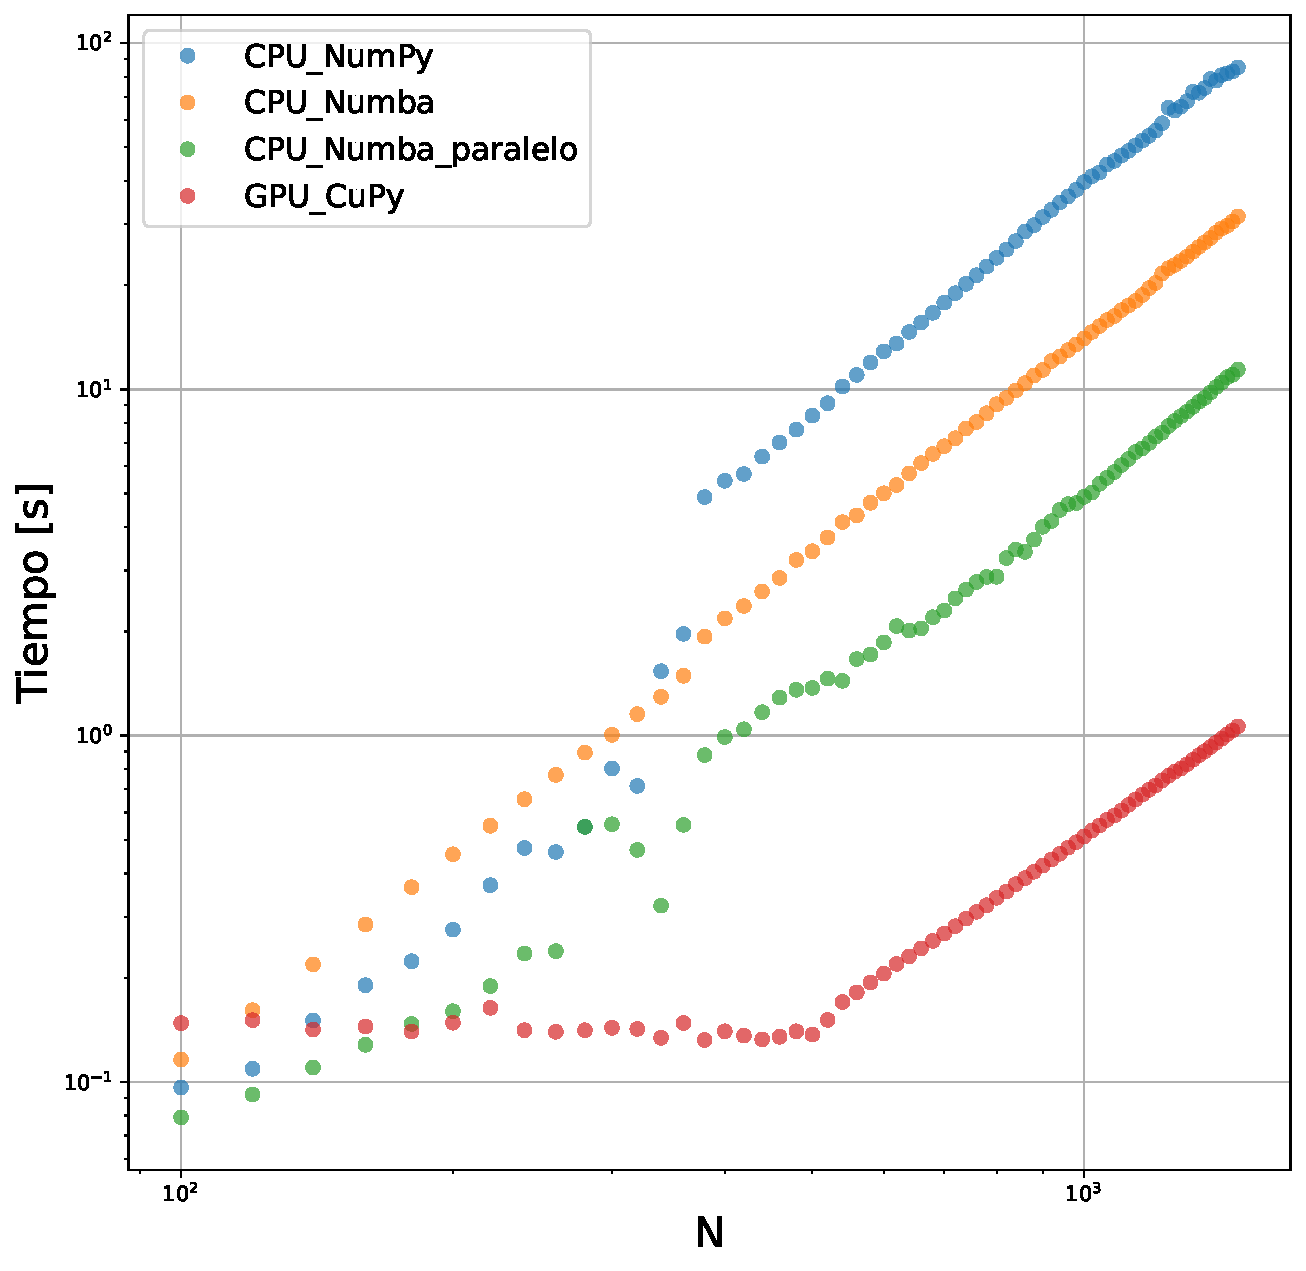
\includegraphics[width=.47\textwidth]{cpu_gpu_t.pdf}
  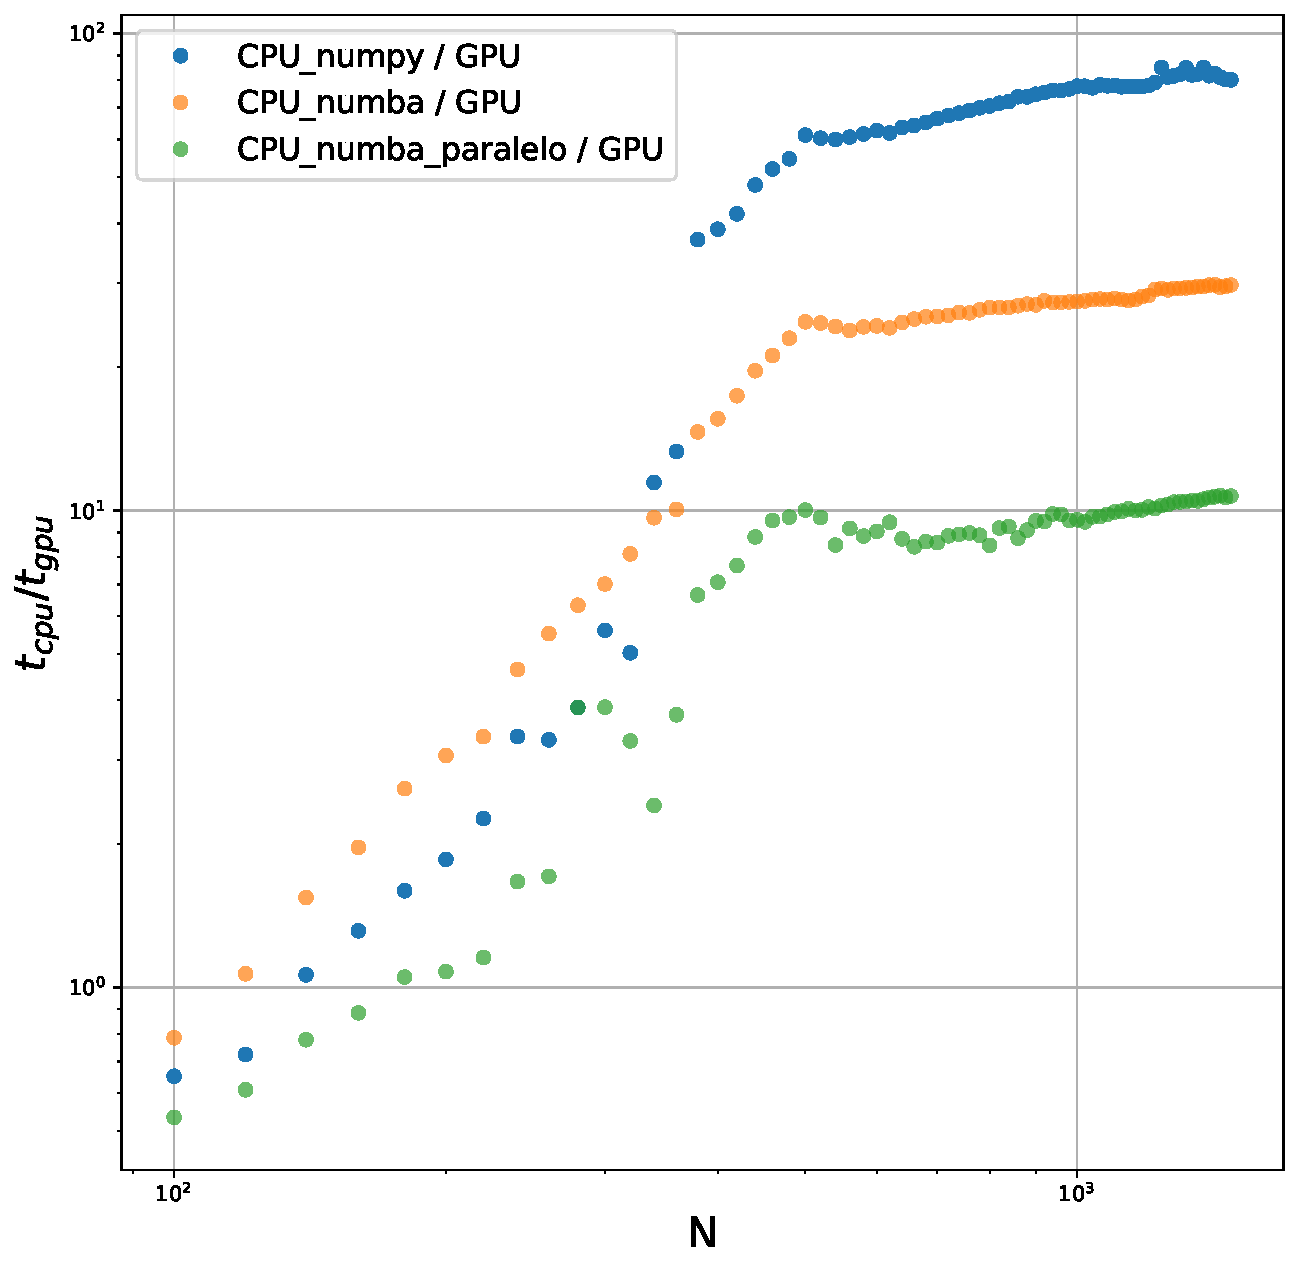
\includegraphics[width=.47\textwidth]{cpu_gpu_ratio.pdf}
  \caption{bla}
  \label{fig:cpuvsgpu}
\end{figure}

Finalmente, es posible que quienes estén más interiorizados con \textit{CUDA} tal vez estén sorprendidos por el carácter superficial con el que 
usamos la GPU aquí. Es decir, cuando escribimos el \textit{kernel} no lo escribimos en \textit{CUDA C} o \textit{CUDA C++}, es algo similar, pero 
es distinto, lo cual puede confundir un poco. Además, en ningún momento indicamos cantidad de hilos por bloque y cantidad de bloques en la 
grilla. Esto es nuevamente, porque \textit{CuPy} intenta simplificar todo lo posible el uso de la GPU, para que sea accesible a usarios sin conocimientos 
de \textit{CUDA}. Sin embargo, \textit{CuPy} ofrece también todo el acceso al detalle, tal como podría hacerse con \textit{CUDA C} por ejemplo,
y admite la escritura de \textit{kernels} directamente en \textit{CUDA C} a través de la función 
\href{https://docs.cupy.dev/en/stable/user_guide/kernel.html}{\textit{cupy.RawKernel}}. En el material complementario de este capítulo, dejo la 
implementación usando esta función que da acceso completo a \textit{CUDA}. No la agrego acá porque entiendo que no aporta demasiado, adicionalemente, no 
pude obtener ninguna mejora notable respecto al \textit{kernel} escrito con \textit{cupy.ElementwiseKernel}. Esto no quiere decir que no se pueda, seguro 
que sí, estuve investigando algunas posibilidad para hacerlo, solo que no me ha dado el tiempo de explorarlas debidamente.












\chap{Reseña numérica y computacional}{code}
\graphicspath{{figs/}}
%\label{chap:code}

La idea de este capítulo es dejar documentación que muestre con claridad el trabajo de investigación y elaboración técnico, a nivel computacional, realizado 
para llevar a cabo este proyecto de tesis. Adicionalmente, está en mi intención ser lo más genérico, claro y acotado posible, para que sea de utilidad a cualquier 
otra persona que esté interesada en resolver ecuaciones diferenciales parciales haciendo uso de programación en paralelo. En particular, usando 
\href{https://developer.nvidia.com/cuda-toolkit}{\textit{CUDA}} a través de las bondades que ofrece \href{https://www.python.org/}{\textit{Python}} mediante 
la librería \href{https://cupy.dev/}{\textit{CuPy}}.

Este capítulo cuenta con un material complementario en formato de \textit{Jupyter Notebook} en \textit{Google Colab} al cual puede acceder desde 
\href{https://colab.research.google.com/drive/13dfbe0GnIngJ2q3w2jLOlSO6mtFYZmA7?usp=sharing}{aquí}. \textit{Google Colab} da acceso gratuito a GPUs,
lo cual está fantástico para aprender a usarlas, aunque evidentemente es con tiempo limitado. En este \textit{Jupyter Notebook} esencialmente 
encontrará todo el código prensentado aquí y un poco más, para que pueda interactuar y hacer las modificaciones que quiera.

A continuación dejamos constancia del \textit{software} y \textit{hardware} utilizado en la ejecución de los códigos de este capítulo.

\begin{itemize}
  \item Python: 3.9.7
  \item CUDA Version: 11.6
  \item CPU: AMD Ryzen 9 5900HX
  \item GPU: NVIDIA GeForce RTX 3060 Laptop
  \item Memoria de GPU: 6GB
  \item CUDA cores: 3840
  \item RAM: 32GB
\end{itemize}

\section{Diferencias finitas}
\label{S:diferencias finitas}

El objetivo es resolver numéricamente ecuaciones diferenciales parciales de la manera más simple y eficiente posible. Para la física este tipo de ecuaciones son de gran 
interés ya que se usan ampliamente para modelar todo tipo de fenómenos. 

Para reducir la complejidad del problema, acotamos la discusión mostrando en detalle el proceso de resolución de un sistema de 
dos ecuaciones de reacción-difusión con dos dimensiones espaciales $(x,y)$ en cierta región $\Omega \in \mathbb{R}^2$. Esto es conveniente porque 
este problema corresponde con el tipo de sistemas usados en este trabajo. Explícitamente, queremos resolver,

\begin{equation}
\begin{split}
 \partial_t u & = f_u(u,v) + D_u \laplacian{u}\\
 \partial_t v & = f_v(u,v) + D_v \laplacian{v}, 
\label{eq:sist_rf}
\end{split}
\end{equation}
donde $u$ y $v$ son las variables dinámicas que dependen de las variables $(t,x,y)$, $f_u$ y $f_v$ son funciones suaves, mientras que $D_u$ y $D_v$ 
son los coeficientes de difusión de $u$ y $v$ respectivamente. Estas ecuaciones deben resolverse teniendo en cuenta determinadas condiciones iniciales y 
de contorno para el problema en cuestión, podemos expresarlas genéricamente de la siguiente manera,

\begin{align*}
u(t = 0,x,y) & = g_u(x,y) & \forall x,y \in \Omega &&|&& u(t,x,y) = h_u(t,x,y) && \forall t\in \mathbb{R};\; \forall x,y \in \delta \Omega\\
v(t = 0,x,y) & = g_v(x,y) & \forall x,y \in \Omega &&|&& v(t,x,y) = h_v(t,x,y) && \forall t\in \mathbb{R};\; \forall x,y \in \delta \Omega.
\label{eq:ic}
\end{align*}
Donde las funciones $g_u$ y $g_v$ denotan las condiciones iniciales del sistema, las funciones $h_u$ y $h_v$ las 
condiciones de contorno y $\delta \Omega$ es el borde de $\Omega$.

De esta manera queda completamente definido el problema y procedemos al armado del esquema numérico necesario para resolverlo. Por simplicidad consideramos que $\Omega$
es una región rectangular del plano donde $x,y \in~[0,L_x] \times~[0,L_y]$. Segmentamos este espacio en $N_x \times N_y$ cuadrantes de dimensiones $d_x = L_x/N_x$ y 
$d_y=L_y/N_y$ y denomminamos $u_{ij}$ y $v_{ij}$ a los valores de las funciones $u$ y $v$ a tiempo $t$ en el cuadrante $(i,j)$ corespondiente a la región 
$[jd_x,(j+1)d_x) \times [id_y,(i+1)d_y)$, con $i =0,1,...,N_y-1$ y $j = 0,1,...,N_x-1$.

A continuación, la idea consiste en reducir el sistema de ecuaciones diferenciales parciales \ref{eq:sist_rf} en un sistema de ecuaciones diferenciales ordinarias, donde 
cada ecuación describe la evolución de las variables dinámicas en un cuadrante distinto. Para ello necesitamos llevar los laplacianos de las ecuaciones al nuevo esquema 
espacial discretizado. Lo hacemos usando la siguiente aproximación por diferencias finitas para los laplacianos,

\begin{equation}
  \begin{split}
    (\laplacian u)_{ij} &= \frac{1}{d^2}(u_{i+1,j}+u_{i-1,j}+u_{i,j+1}+u_{i,j-1}-4u_{ij})\\
    (\laplacian v)_{ij} &= \frac{1}{d^2}(v_{i+1,j}+v_{i-1,j}+v_{i,j+1}+v_{i,j-1}-4v_{ij})
    \label{eq:lap}
  \end{split}
\end{equation}
donde usamos que $d = d_x = d_y$.  Utilizando la notación dada para la discretización espacial, tenemos el siguiente sistema 
de ecuaciones diferenciales ordinarias,

\begin{equation}
  \begin{split}
  \dv{u_{ij}}{t} & = f_u(u_{ij},v_{ij}) + D_u (\laplacian u)_{ij} \\
  \dv{v_{ij}}{t} & = f_v(u_{ij},v_{ij}) + D_v (\laplacian v)_{ij}.
  \label{eq:sist_ord}
  \end{split}
\end{equation}

Finalmente, discretizamos el espacio temporal con un intervalo $dt$ y aproximamos la derivada temporal a primer orden. Usando $n\in \mathbb{N}$ como ínidce temporal, notamos $u_{ij}^n$ 
y $v_{ij}^n$ como el valor de las funciones $u$ y $v$ en el instante $t = n*dt$ sobre el cuadrante $(i,j)$. De esta manera obtenemos el siguiente 
esquema explícito de Euler para la resolución numérica del sistema \ref{eq:sist_rf},

\begin{equation}
  \begin{split}
    u_{ij}^{n+1} & = u_{ij}^n + dt \, \left(f_u(u_{ij}^n,v_{ij}^n) + D_u (\laplacian u)_{ij}^n\right) \\
    v_{ij}^{n+1} & = v_{ij}^n + dt \, \left(f_v(u_{ij}^n,v_{ij}^n) + D_v (\laplacian v)_{ij}^n\right),  
    \label{eq:euler}
  \end{split}
\end{equation}
a partir del cual podemos iterar para obtener la solución. En la siguiente sección se decribe cómo hacer esto usando \textit{Python} con diferentes niveles de eficiencia.


\section{Implementaciones en \textit{Python}}
\label{S:Python}

En esta sección se describen brevemente 4 implementaciones distintas para la resolución del esquema numérico \ref{eq:euler} hayado en la sección anterior. Comenzamos por 
la más ineficiente, que correponde con el uso de la librería \href{https://numpy.org/}{\textit{NumPy}} en un esquema serial (mucho peor aún es \textit{Python} nativo, pero vamos a saltearnos este caso), 
hasta llegar a la más eficiente obtenida, correspondiente a la utilización de \textit{CUDA} a través de la librería \textit{CuPy}. 

La razón para hacer esto reside nuevamente en la idea de dejar documentación que pueda llegar a ser de utilidad para alguien más lidiando 
con problemas de índole numérico donde la eficiencia de la resolución es relevante. Además, antes de llegar a la versión final, donde usamos \textit{CUDA} y 
consecuentemente es necesario un procesador gráfico (GPU) compatible con \textit{CUDA}, se muestran implementaciones que son notablemente eficientes sin necesidad 
de un GPU, y que pueden ser usadas por una computadora más modesta.

\subsection{Implementación con \textit{NumPy}}
\label{SS:NumPy}
\textit{NumPy} es una de las librerias fundamentales para hacer computación científica en \textit{Python}. Ofrece los invaluables \textit{NumPy Arrays}, que están diseñados 
específicamente para ser lo más eficiente posible en la manipulación numérica sin perder la simplicidad y elegancia de \textit{Python}. Utilizando \textit{NumPy} 
se obtienen mejores resultados que usando \textit{Python} nativo porque integra código de \textit{C,C++ y Fortran} dentro de \textit{Python}, adicionalmente la mayoría 
de los métodos implementados para la operación con \textit{NumPy arrays} están paralelizados.

El código \ref{lst:NumPy} muestra la implementación propuesta usando \textit{NumPy}. Nótese que hay más líneas de comentarios que de código. Esencialemente, 
primero definimos una función que llamamos \textit{laplacian}, que toma un \textit{array} 2D 
y devuelve su laplaciano, para ello usamos la función \textit{roll} de \textit{NumPy} que desplaza un \textit{array} sobre un eje dado
cuanto queramos y con condiciones periódicas.
Luego, sumamos y restamos estas matrices desplazadas según \ref{eq:lap} y obtenemos el laplaciano. Finalmente, definimos la función \textit{cpu\_numpy\_solver}, que toma 
por argumentos las condiciones iniciales del problema, las funciones de reacción $f_u$ y $f_v$, los coeficientes de difusión, 
el intervalo de integración temporal $dt$ y espacial $d$ y la cantidad de iteraciones $it$. 

\begin{lstlisting}[language=Python,caption = Implementación con NumPy.,label = {lst:NumPy}]
import numpy as np

def laplacian(X):
  '''
  Take the Laplacian of a 2D array with periodic boundary conditions.
  '''
  return np.roll(X,1,axis = 0) + np.roll(X,-1,axis = 0) + np.roll(X,1,axis = 1) + np.roll(X,-1,axis = 1) - 4*X

def cpu_numpy_solver(u, v, fu, fv, Ds, dt = .01, d = 1, it = 1000):
  '''
  Solve a 2D reaction-diffusion equation for two dynamical variables with periodic boundary conditions using NumPy.

  u: Intial conditions for the first dynamical variable. 2d NumPy array.
  v: Intial conditions for the second dynamical variable. 2d NumPy array.
  fu: Reaction term for the first dynamical variable. Function.
  fv: Reaction term for the second dynamical variable. Function.
  Ds: Diffusion coefficients for the first and second dynamical variables. List or array of length 2.
  dt: Time step. Default value is 0.01.
  d: Space step. Default value is 1.
  it: Number of iterations. Default value is 1000.
  '''
  
  Du,Dv = Ds
  for _ in range(it):
      u = u + dt*(fu(u,v) + Du*laplacian(u)/d**2)
      v = v + dt*(fv(u,v) + Dv*laplacian(v)/d**2)

  return u,v

\end{lstlisting}


\begin{lstlisting}[language=Python, caption = Ejemplo de uso de la implementación con \textit{NumPy}.,label = {lst:numpy_ex}]
def fu(u,v,beta):
  return -beta*u*v

def fv(u,v,beta,gamma):
  return beta*u*v - gamma*v

L = 1024
beta = 1
gamma = .2
u = np.ones((L,L))
v = np.zeros((L,L))
u[:,0] = 0
v[:,0] = 1
Ds = [0,1]

uf,vf = cpu_numpy_solver(u,v,fu,fv,Ds)
\end{lstlisting}
En el código \ref{lst:numpy_ex} se muestra un ejemplo de uso utilizando las siguientes funciones de reacción,

\begin{equation}
  \begin{split}
    f_u(u,v) &= -\beta u v,\\
    f_v(u,v) &= \beta uv - \gamma v,\\
  \end{split}
\end{equation}
donde $\beta$ y $\gamma$ son constantes.

Finalmente, a continuación se muestra la velocidad de la resolución con un sistema de $1024\times 1024$ utilizando todos los parámetros y funciones 
del ejemplo \ref{lst:numpy_ex}. Para una justa comparación con las demás implementaciones, utilizaremos exactamente los mismos parámetros y funciones.
\begin{lstlisting}[language=Python,label = {lst:numpy_re}]
  %timeit cpu_numpy_solver(u,v,fu,fv,Ds)
  1min +- 1.53 s per loop (mean +- std. dev. of 7 runs, 1 loop each)
\end{lstlisting}

\subsection{Implementación serial con \textit{Numba}}

Otra de las librerías fundamentales para cálculo numérico en \textit{Python} es \href{https://numba.pydata.org/}{\textit{Numba}}. \textit{Numba} toma código 
nativo de \textit{Python} y genera código de máquina optimizado usando \href{https://llvm.org/}{\textit{LLVM compiler infrastructure}}. También es capaz de 
procesar \textit{NumPy} con una gran cantidad de sus métodos.\footnote{Para ver más detalles consultar la 
\href{https://numba.readthedocs.io/en/stable/reference/numpysupported.html}{documentación de \textit{Numba}}.} 

Lo mejor de todo esto es que \textit{Numba} lo hace de manera completamente autónoma, solo hay que decirle que lo haga. Para ello utilizamos el decorador 
\textit{@njit}, que indica a \textit{Numba} que la función en cuestión debe ser procesada. El código \ref{lst:numba} muestra cómo sería la 
implementaciones en este caso. Se define la función \textit{cpu\_numba\_solver} que toma los mismos argumentos que la función \textit{cpu\_numpy\_solver} 
vista anteriormente. Dentro de la función iteramos temporalmente y para calcular los laplacianos y términos de reacción en cada cuadrante
recorremos las matrices con un ciclo \textit{for}. Usualmente es posible 
tomar las funciones o implementaciones realizadas con \textit{Numpy} y decorarlas con \textit{@njit} para obtener el resultado deseado. Sin embargo, 
en este caso no podemos hacerlo con las funciones del código \ref{lst:NumPy} porque \textit{Numba} no soporta la función \textit{roll} de \textit{NumPy}. Por 
lo cual estamos forzados a calcular el laplaciano de una manera más explicita para que \textit{Numba} lo entienda.    

\begin{lstlisting}[language=Python,caption = Implementación serial con \textit{Numba}.,label = {lst:numba}]
from numba import njit
import numpy as np

@njit()
def cpu_numba_solver(u, v, fu, fv, Ds, dt=.01, d = 1, it = 1000):
  '''
  Solve a 2D reaction-diffusion equation for two dynamical variables with periodic boundary conditions using Numba 
  in a serial implementation.

  u: Intial conditions for the first dynamical variable. 2d NumPy array of shape (Ly,Lx).
  v: Intial conditions for the second dynamical variable. 2d NumPy array of shape (Ly,Lx).
  fu: Reaction term for the first dynamical variable. Function.
  fv: Reaction term for the second dynamical variable. Function.
  Ds: Diffusion coefficients for the first and second dynamical variables. List or array of length 2.
  dt: Time step. Default value is 0.01.
  d: Space step. Default value is 1.
  it: Number of iterations. Default value is 1000.
  '''    

  Ly,Lx = u.shape
  u = u.reshape(Ly*Lx)
  v = v.reshape(Ly*Lx)
  Fu = np.zeros_like(u)
  Fv = np.zeros_like(v)
  Du,Dv = Ds
  for _ in range(it):
    for i in range(Lx*Ly):
      x = i % Lx
      y = i // Lx
      Lu = (u[(x+1)%Lx + Lx*y] + u[(x-1+Lx)%Lx+Lx*y] + u[x + Lx*((y+1)%Ly)] + u[x + Lx*((y-1+Ly)%Ly)] - 4*u[i])/d**2
      Lv = (v[(x+1)%Lx + Lx*y] + v[(x-1+Lx)%Lx+Lx*y] + v[x + Lx*((y+1)%Ly)] + v[x + Lx*((y-1+Ly)%Ly)] - 4*v[i])/d**2
      Fu[i] = fu(u[i],v[i]) + Du*Lu 
      Fv[i] = fv(u[i],v[i]) + Dv*Lv
    u = u + dt*Fu
    v = v + dt*Fv
  return u.reshape(Ly,Lx),v.reshape(Ly,Lx) 
\end{lstlisting}

En cuanto al ejemplo de uso, sería idéntico al mostrado en \ref{lst:numpy_ex}, con la única salvedad de que las funciones $f_u$ y $f_v$ también deben estar decoradas 
con \textit{@njit}. A continuación se muestra el tiempo de resolución para sistemas de $1024\times1024$ en esta versión. Resulta cerca de 3 veces más rápido 
que \ref{lst:NumPy}.

\begin{lstlisting}[language=Python,label = {lst:numba_re}]
%timeit cpu_numba_solver(u,v,fu,fv,Ds)
18.1 s +- 564 ms per loop (mean +- std. dev. of 7 runs, 1 loop each)
\end{lstlisting}

\subsection{Implementación paralela con \textit{Numba}}

En esta ocasión la idea es utilizar \textit{Numba} aprovechando que una parte del algoritmo se puede realizar en paralelo. Esto simplemente quiere decir que 
hay un conjunto de operaciones que puede realizarse en simultáneo en lugar de una por una. Este es el caso para el ciclo \textit{for} que se utiliza 
para calcular los laplacianos y términos de reacción en cada cuadrante. Es decir, no es necesario calcular el valor correspondiente al cuadrante $(i,j)$ para 
luego calcular el del cuadrante $(i',j')$, se pueden calcular simultáneamente, en paralelo.

Lo mejor del caso, nuevamente, es que podemos indicarle de una manera muy sencilla a \textit{Numba} que determinado \textit{for} es paralelizable y listo,
\textit{Numba} se encargará de darle las instrucciones en paralelo al procesador. Para ello, todo lo que tenemos que hacer es importar la función \textit{prange}
de \textit{Numba} que sirve para indicarle a \textit{Numba} que el ciclo \textit{for} es paralelizable y pasar la opción \textit{parallel = True} al decorador 
\textit{@njit}. Por completitud mostramos el código de la función \textit{cpu\_numba\_parallel\_solver} en \ref{lst:numba_p}, pero las únicas diferencias con 
la versión serial \ref{lst:numba} son las indicadas aquí.

\begin{lstlisting}[language=Python,caption = Implementación paralela con \textit{Numba}.,label = {lst:numba_p}]
from numba import njit,prange
import numpy as np

@njit(parallel = True)
def cpu_numba_parallel_solver(u, v, fu, fv, Ds, dt=.01, d = 1, it = 1000):
  '''
  Solve a 2D reaction-diffusion equation for two dynamical variables with periodic boundary conditions using Numba 
  with a parallel implementation.

  u: Intial conditions for the first dynamical variable. 2d NumPy array of shape (Ly,Lx).
  v: Intial conditions for the second dynamical variable. 2d NumPy array of shape (Ly,Lx).
  fu: Reaction term for the first dynamical variable. Function.
  fv: Reaction term for the second dynamical variable. Function.
  Ds: Diffusion coefficients for the first and second dynamical variables. List or array of length 2.
  dt: Time step. Default value is 0.01.
  d: Space step. Default value is 1.
  it: Number of iterations. Default value is 1000.
  '''   

  Ly,Lx = u.shape
  u = u.reshape(Ly*Lx)
  v = v.reshape(Ly*Lx)
  Fu = np.zeros_like(u)
  Fv = np.zeros_like(v)
  Du,Dv = Ds
  
  for _ in range(it):
    for i in prange(Lx*Ly):
      x = i % Lx
      y = i // Lx
      L_u = (u[(x+1)%Lx + Lx*y] + u[(x-1+Lx)%Lx+Lx*y] + u[x + Lx*((y+1)%Ly)] + u[x + Lx*((y-1+Ly)%Ly)] - 4*u[i])/d**2
      L_v = (v[(x+1)%Lx + Lx*y] + v[(x-1+Lx)%Lx+Lx*y] + v[x + Lx*((y+1)%Ly)] + v[x + Lx*((y-1+Ly)%Ly)] - 4*v[i])/d**2
      Fu[i] = fu(u[i],v[i]) + Du*L_u 
      Fv[i] = fv(u[i],v[i]) + Dv*L_v
    u = u + dt*Fu
    v = v + dt*Fv
  return u.reshape(Ly,Lx),v.reshape(Ly,Lx)
\end{lstlisting}

A continuación mostramos el rendimiento obtenido con esta nueva versión, observamos que es cerca de 3 veces más rápido que la versión serial \ref{lst:numba} y 
10 veces más rápido que la versión de \textit{NumPy} \ref{lst:NumPy}. Esto muestra una primera aproximación al poder de la programación en paralelo y cómo es 
posible implementarla sin la necesidad de una GPU que naturalemente provee una arquitectura diseñada específicamente para hacer operaciones en paralelo de manera 
masiva.

\begin{lstlisting}[language=Python,label = {lst:numba_p_re}]
%timeit cpu_numba_parallel_solver(u,v,fu,fv,Ds)
6.31 s +- 439 ms per loop (mean +- std. dev. of 7 runs, 1 loop each)
\end{lstlisting}

\subsection{Implementación con \textit{CuPy}}

\textit{CuPy} es una librería de código abierto desarrollada para facilitar el acceso a las GPU compatibles con \textit{CUDA}\footnote{Está en fase experimental la posibilidad 
de usar GPUs con \href{https://rocmdocs.amd.com/en/latest/}{ROCm}.} en \textit{Python}. \textit{Cupy} ofrece prácticamente todos los métodos de 
\textit{NumPy} y se encarga de lidiar de forma autónoma y eficiente con el problema de pasar las instrucciones a la GPU. Esta característica por sí 
sola ya es sorprendente, dado que ofrece la posibilidad de explotar las capacidades de la GPU sin saber nada de CUDA. Ello quiere decir, que en muchos 
casos basta escrbir el código tal como lo haríamos con \textit{NumPy} pero usando \textit{CuPy}, y eso bastaría para tener una mejora decisiva en la 
eficiencia. De hecho, hagamos la prueba, si tomamos el código \ref{lst:NumPy} y lo único que hacemos es cambiar \textit{NumPy} por \textit{CuPy}, el 
resultado obtenido es el siguiente.

\begin{lstlisting}[language=Python,label = {lst:cupy}]
%timeit gpu_simple_cupy_solver(u,v,fu,fv,Ds)
3.12 s +- 3.51 ms per loop (mean +- std. dev. of 7 runs, 1 loop each)
\end{lstlisting}

Esto es cerca de 19 veces más rápido que la versión de \textit{NumPy} y además la más rápida hasta ahora, lograda con un esfuerzo mínimo. Cabe recordar que 
el tamaño del sistema que estamos resolviendo, es de $1024\times1024$ en todos los casos, este es un terreno favorable para el uso de GPU, dado que 
es un sistema lo suficientemente grande como para que la capacidad de paralelización másiva de la GPU marque la diferencia. Esto es de carácter elemental 
en lo que respecta al uso de procesadores gráficos para cálculo numérico, sin embargo no está de más recordarlo. No siempre es preferible usar la GPU,
hay que ponderar el carácter del algoritmo a utilizar y la magnitud de operaciones susceptibles de ser paralelizadas. Si corremos los mismos códigos 
con un sistema de $100\times100$, las cosas cambian rotundamente.
\begin{lstlisting}[language=Python,label = {lst:cupy}]
#Sistemas de 100x100
#Numpy
%timeit cpu_numpy_solver(u,v,fu,fv,Ds)
163 ms +- 502 us per loop (mean +- std. dev. of 7 runs, 10 loops each)
#Cupy
%timeit gpu_simple_cupy_solver(u,v,fu,fv,Ds)
1.07 s +- 3.91 ms per loop (mean +- std. dev. of 7 runs, 1 loop each)
\end{lstlisting}

Ahora bien, volviendo a sistemas grandes, podría decirse que una mejora en un factor $19$ es sorprendente, sin embargo esto es así solo si comparamos
con la implementación de \textit{NumPy}, pero si miramos la mejora respecto de la implementación con \textit{Numba} en paralelo, el factor de 
mejora es cerca de $2$. En este caso alguien podría decir, con razón, que la utilización de la \textit{GPU} no está justificada, dado que la 
mejora en eficiencia no vale el costo que implica el acceso a la GPU.  

Para sortear esta razonable objeción, solo debemos profundizar un poco más en las herramientas que nos ofrece \textit{CuPy}. Como decíamos al principio, 
el hecho de que \textit{CuPy} ofrezca la posibilidad de acceder a la computación en GPU de una manera extremadamente sencilla y con buenos resultados, es 
sorprendente. Sin embargo, como es habitual, esa sencillez no viene gratis, paga un peaje a la potencia de cómputo real que puede ofrecer una GPU. 

En lo que sigue se muestra cómo es posible sacar más provecho de la GPU, sin salirnos del entorno que ofrece \textit{CuPy}. La razón por la que estamos 
desperdiciando potencia de cómputo al resolver el problema reemplazando \textit{CuPy} por \textit{NumPy} es porque estamos lanzando demasiados 
\textit{kernels} de manera de innecesaria. Es radicalmente más eficiente si conseguimos juntar todas las operaciones necesarias en una menor 
cantidad de \textit{kernels}. Por cierto, se le dice \textit{kernel} a una función que se ejecuta en la GPU, comúnmente esta función 
representan operaciones elementales que se realizan en paralelo en la GPU. Para entender esto, vamos a ver un ejemplo sencillo antes de atacar el 
problema original.

Supongamos que queremos multiplicar las matrices $A$ y $B$, elemento a elemento, y luego sumar el resultado a la matriz $C$. Utilizando 
\textit{CuPy arrays} la función en cuestión y el resultado obtenido es el siguiente.

\begin{lstlisting}[language=Python,label = {lst:sum_add}]
import cupy as cp
def mul_add(A,B,C):
    return A*B + C

L = 1024
A = cp.ones((L,L))
B = cp.ones((L,L))
C = cp.ones((L,L))
mul_add(A,B,C)
%timeit mul_add(A,B,C)
215 us +- 6.81 us per loop (mean +- std. dev. of 7 runs, 1,000 loops each)
\end{lstlisting}

Ahora bien, podemos hacerlo mejor, el problema con la función anterior es que está utilizando dos \textit{kernels} en lugar de uno, uno para multiplicar 
y el otro para sumar. Sin embargo sería mejor si pudieramos usar un solo \textit{kernel} que hiciera las dos cosas a la vez. Para ello, \textit{CuPy} 
ofrece la posibilidad de escribir \textit{kernels} personalizados, una de las maneras de hacerlo, es utilizando la función \textit{cupy.ElementwiseKernel}.
A continuación se muestra cómo quedaría la función y su resultado utilizando esta alternativa.

\begin{lstlisting}[language=Python,label = {lst:sum_add_kernel}]
import cupy as cp
mul_add_kernel = cp.ElementwiseKernel(
  'float64 A, float64 B, float64 C', 'float64 out',
  'out = A*B + C', 'mul_add')
  
L = 1024
A = cp.ones((L,L))
B = cp.ones((L,L))
C = cp.ones((L,L))
mul_add_kernel(A,B,C)
%timeit mul_add_kernel(A,B,C)
136 us +- 273 ns per loop (mean +- std. dev. of 7 runs, 10,000 loops each)
\end{lstlisting}
Vemos que la velocidad aumentó apreciablemente aún en un ejemplo tan sencillo como este, si aplicamos esta misma idea a algoritmos más 
complejos tenemos la posibilidad de mejorar la eficiencia sorprendentemente. No voy a entrar en los detalles de utilización de la función 
\textit{cupy.ElementwiseKernel}, para más detalles recomiendo la siguiente \href{https://docs.cupy.dev/en/stable/user_guide/kernel.html}{documentación}.

Ahora procedemos finalmente con la propuesta para la resolución del problema original usando esta nueva idea de fusionar \textit{kernels} 
(Código \ref{lst:CuPy}). Para ello lo que haremos será concentrar en un único \textit{kernel} los cálculos necesarios para evaluar las funciones 
de reacción y los laplacianos. Nuevamente, no me dentendré a explicar los detalles de la implementación, pero espero que el código sea lo suficientemente
claro como para motivar el interés del lector.

\begin{lstlisting}[language=Python,caption = Implementación con \textit{CuPy}.,label = {lst:CuPy}]
import cupy as cp

forces = cp.ElementwiseKernel(
  'raw float64 u, raw float64 v, float64 beta, float64 gamma, float64 Du, float64 Dv, uint32 Lx, uint32 Ly',
  'float64 Fu, float64 Fv',
  '''
  int x = i % Lx;
  int y = (int) i / Lx;
  Fu = -beta*u[i]*v[i] + Du*(u[(x+1)%Lx+Lx*y] + u[(x-1+Lx)%Lx+Lx*y] + u[x+Lx*((y+1)%Ly)] + u[x+Lx*((y-1+Ly)%Ly)]
        - 4*u[i]);
  Fv = beta*u[i]*v[i] - gamma*v[i] + Dv*(v[(x+1)%Lx + Lx*y] + v[(x-1+Lx)%Lx+Lx*y] + v[x + Lx*((y+1)%Ly)] 
        + v[x + Lx*((y-1+Ly)%Ly)] - 4*v[i]);
  ''',
  'forces')

euler = cp.ElementwiseKernel(
  'float64 Fu, float64 Fv, float64 dt','float64 u, float64 v',
  '''
  u = u + dt*Fu;
  v = v + dt*Fv;
  ''',
  'euler')

def gpu_cupy_solver(u, v, Ds, beta = 1.,gamma = .2, dt = .01, d = 1, it = 1000):
  '''
  Solve a 2D reaction-diffusion equation for two dynamical variables with periodic boundary conditions using CuPy.

  u: Intial conditions for the first dynamical variable. 2d CuPy array of shape (Ly,Lx).
  v: Intial conditions for the second dynamical variable. 2d CuPy array of shape (Ly,Lx).
  Ds: Diffusion coefficients for the first and second dynamical variables. List or array of length 2.
  dt: Time step. Default value is 0.01.
  d: Space step. Default value is 1.
  it: Number of iterations. Default value is 1000.
  ''' 
  Ly,Lx = u.shape
  Du,Dv = Ds
  Fu = cp.zeros_like(u)
  Fv = cp.zeros_like(v)

  for _ in range(it):
    forces(u,v,beta,gamma,Du,Dv,Lx,Ly,Fu,Fv)
    euler(Fu,Fv,dt,u,v)
  return u,v
\end{lstlisting}

Este es el tipo de implementación utilizada en este proyecto de tesis, el resultado obtenido en esta ocasión es el siguiente,
\begin{lstlisting}[language=Python]
  %timeit gpu_cupy_solver(u,v,Ds)
  511 ms +- 12.3 ms per loop (mean +- std. dev. of 7 runs, 1 loop each)
\end{lstlisting}
esto es, mejor en un factor $6$ que la versión estándar de \textit{CuPy}, 12 veces mejor que la implementación con \textit{Numba} en paralelo 
(la mejor sin usar GPU), y 117 veces más rápido que la versión con \textit{NumPy}. Ahora sí, vemos que la diferencia entre usar una GPU y no usarla es, 
por lo menos, en un factor de 12, la diferencia entre una simulación de un 1 día  y una de 12 días.

Por último, quisiera terminar este capítulo con algunos comentarios. Por un lado, recordar que todas las comparaciones de velocidad en las diferentes 
implementaciones se realizaron con los mismos parámetros, y fundamentalmente con sistemas relativamente grandes, $1024\times1024$, donde la GPU se ve 
favorecida sobre la CPU. Diferente es el caso para sistemas chicos, por completitud en este sentido, en la figura \ref{fig:cpuvsgpu} mostramos 
los resultados de velocidad de las distintas implementaciones para distintos tamaños de sistemas. Por otro lado, la mayoría de los resultados presentados  
en este proyecto fueron obtenidos con sistemas de $2^{16} \times 2^{11}$, en un sistema de dos ecuaciones de reacción-difusión como el discutido aquí,
esto implica cuatro matrices con $2^{27}$ elementos cada una, considerando que además utilizamos un formato en coma flotante de doble precisión, cada 
matriz ocupa alrededor de $1GB$ de memoria. El tiempo que llevaría resolver sistemas de este tamaño sin GPU sería completamente inviable. 

\begin{figure}[h]
  \centering
  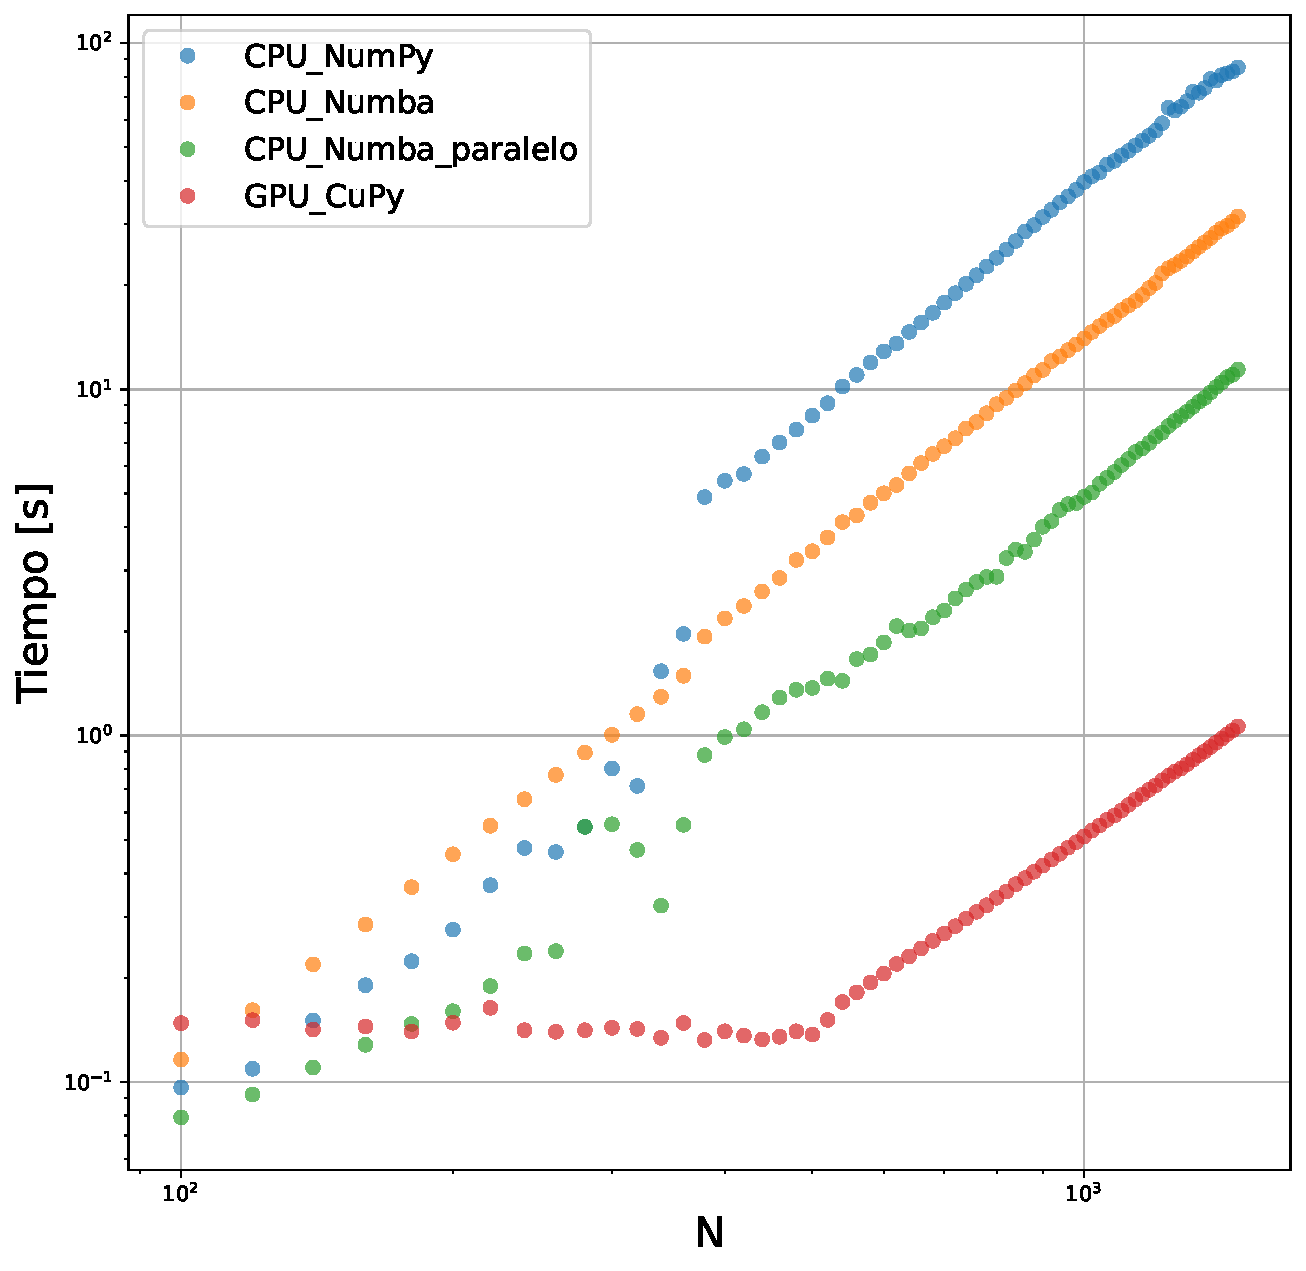
\includegraphics[width=.47\textwidth]{cpu_gpu_t.pdf}
  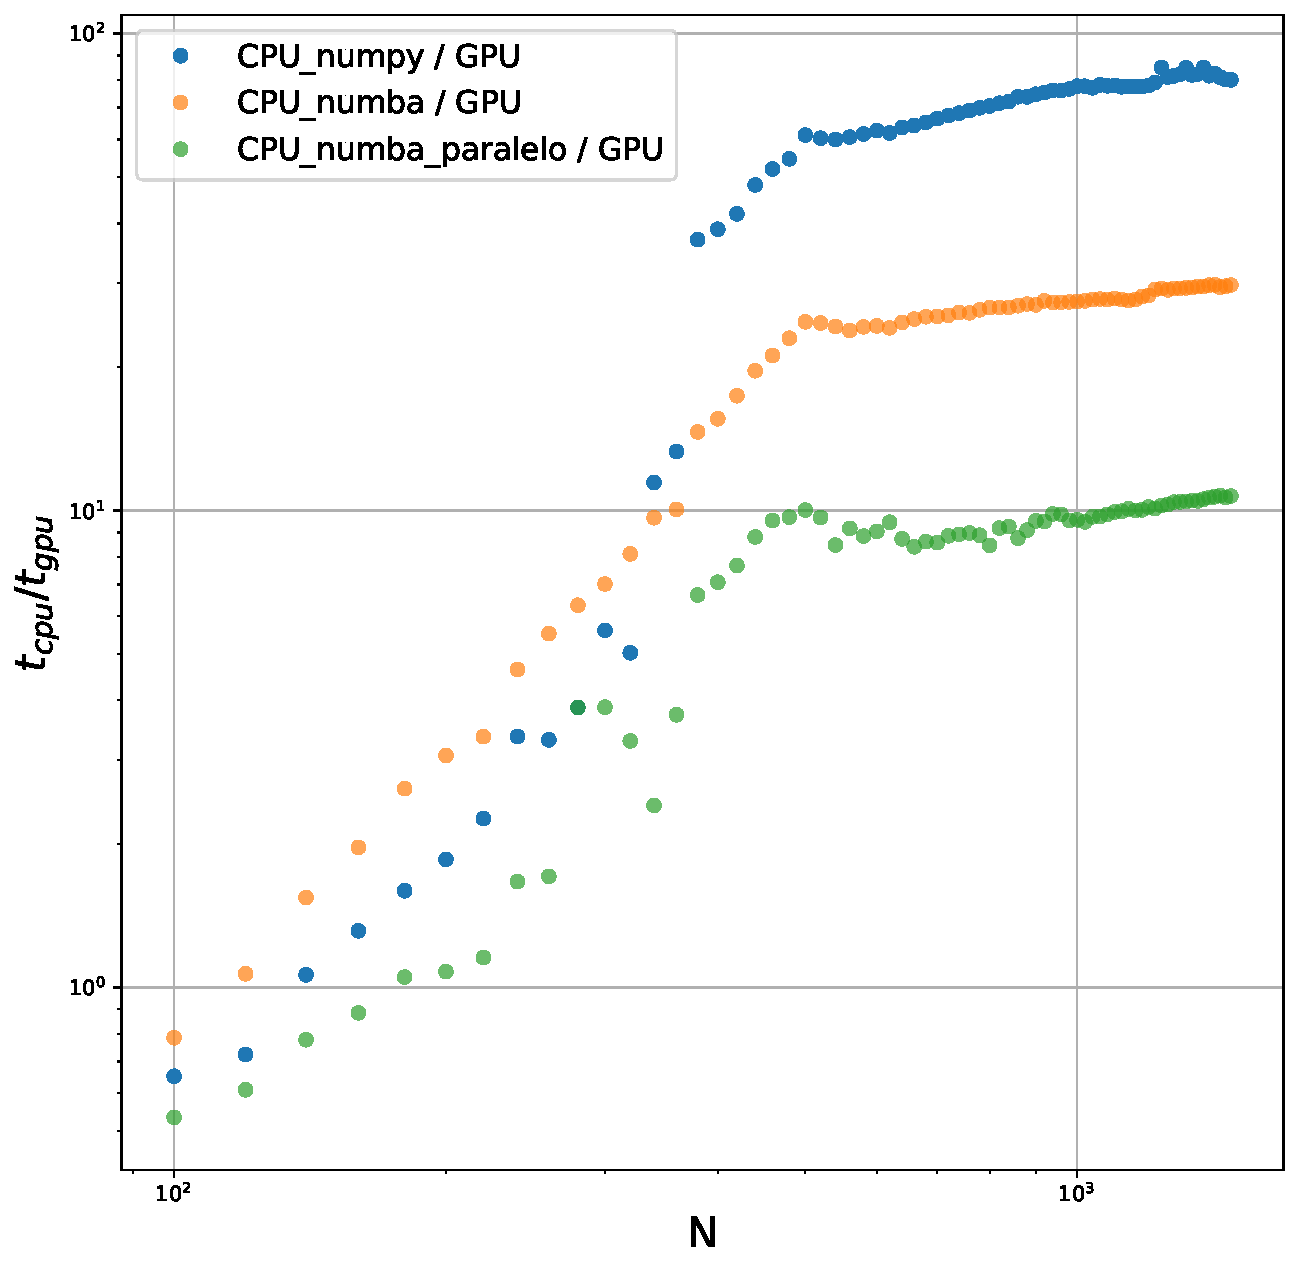
\includegraphics[width=.47\textwidth]{cpu_gpu_ratio.pdf}
  \caption{bla}
  \label{fig:cpuvsgpu}
\end{figure}

Finalmente, es posible que quienes estén más interiorizados con \textit{CUDA} tal vez estén sorprendidos por el carácter superficial con el que 
usamos la GPU aquí. Es decir, cuando escribimos el \textit{kernel} no lo escribimos en \textit{CUDA C} o \textit{CUDA C++}, es algo similar, pero 
es distinto, lo cual puede confundir un poco. Además, en ningún momento indicamos cantidad de hilos por bloque y cantidad de bloques en la 
grilla. Esto es nuevamente, porque \textit{CuPy} intenta simplificar todo lo posible el uso de la GPU, para que sea accesible a usarios sin conocimientos 
de \textit{CUDA}. Sin embargo, \textit{CuPy} ofrece también todo el acceso al detalle, tal como podría hacerse con \textit{CUDA C} por ejemplo,
y admite la escritura de \textit{kernels} directamente en \textit{CUDA C} a través de la función 
\href{https://docs.cupy.dev/en/stable/user_guide/kernel.html}{\textit{cupy.RawKernel}}. En el material complementario de este capítulo, dejo la 
implementación usando esta función que da acceso completo a \textit{CUDA}. No la agrego acá porque entiendo que no aporta demasiado, adicionalemente, no 
pude obtener ninguna mejora notable respecto al \textit{kernel} escrito con \textit{cupy.ElementwiseKernel}.












%\chap{Modelo SIR}{SIR}
\graphicspath{{figs/cap3}}

\sect{Historia}{historia}

Desde tiempos remotos las epidemias y pandemias han sido origen de sufrimiento para la humanidad. Cada individuo, pueblo, ciudad o civilización amenazada por una epidemia ha tenido 
que enfrentarlas de una u otra manera. La historia de la humanidad está llena de acontecimientos epidemiológicos que han causado grandes pérdidas de vidas humanas y cambios en la 
forma de vida de las sociedades. La peste negra, la gripe española, la viruela, la tuberculosis, la malaria  y la fiebre amarilla,
entre otras, han sido algunas de las epidemias más devastadoras de la historia. 

A continuación haremos un breve repaso histórico de dos de las epidemias mencionadas arriba, la peste negra y la gripe española. Destacaremos algunos detalles de cada una de 
ellas para ilustrar la complejidad dinámica de las epidemias y la cantidad de detalles que debe tenerse en cuenta a la hora de modelarlas. Además, dados los recientes 
acontecimientos epidemiológicos, creo que resulta de interés poner en observación algo de la extensa historia epidemiológica de la humanidad.

\subsection*{Peste Negra}

En la Edad Media, la Peste Negra, fue una epidemia de peste bubónica que se extendió por Europa entre 1347 y 1350, causando la muerte de entre un tercio y la mitad de la 
población europea \cite{black_death3}. La enfermedad era producida por la bacteria \textit{Yersinia pestis}, que se transmitía por la picadura de pulgas infectadas. De hecho, el mecanismo de 
transmisión de la enfermedad fue un misterio durante mucho tiempo.
En 1855, una epidemia de peste bubónica, ocasionda por la misma bacteria responsable de la peste negra, comenzó en el sur de China. Fue entonces cuando pudieron obtenerse resultados de laboratorio y recién en 1897, M. Ogata, y en 1898,
P. L. Simonds, de manera independiente llegaron a la hipótesis de que la enfermedad se transmitía por medio de la picadura de pulgas infectadas. Lo cual fue confirmado unos 
años más tarde. 

\begin{figure}[!b]
    \centering
    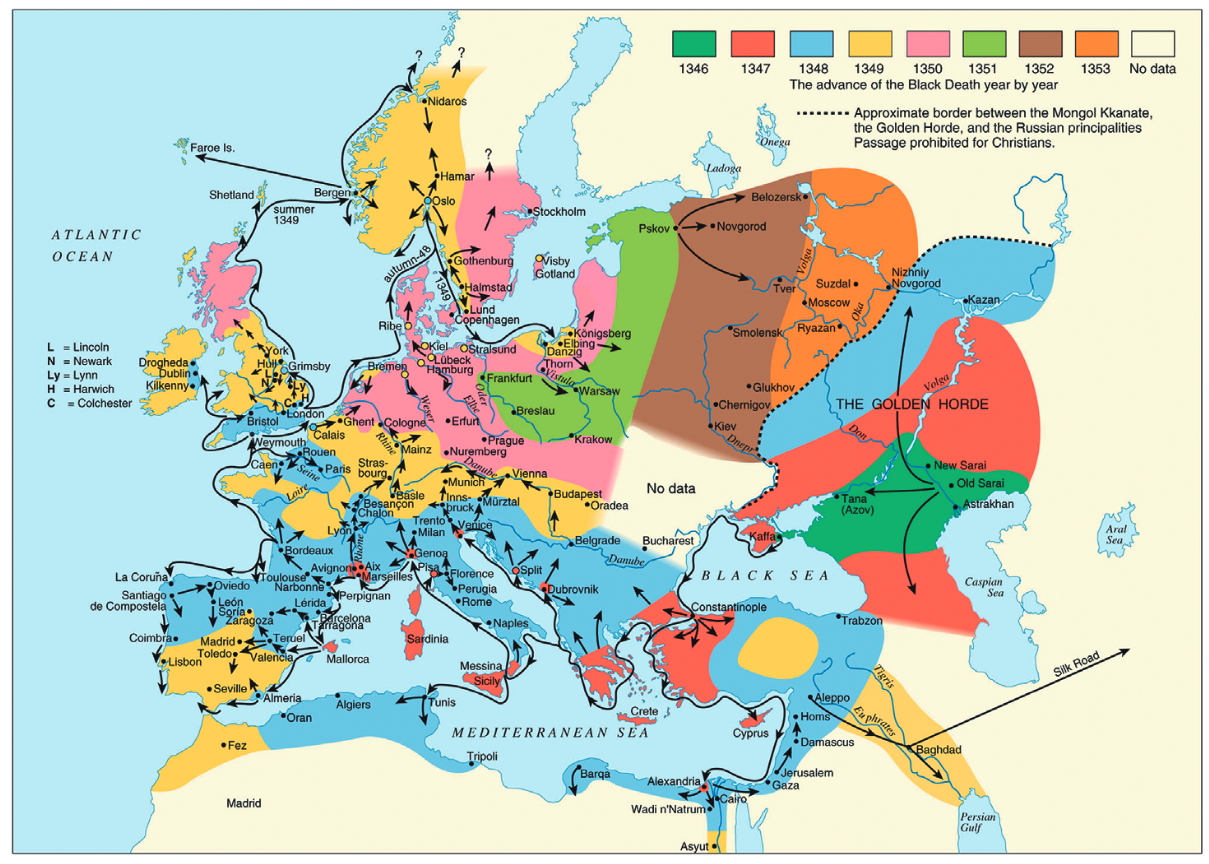
\includegraphics[width=\imsizeL]{Black_Death.png}
    \caption[Evolución de la peste negra en Europa.]{Evolución de la peste negra en Europa. Figura extraída de Ref. \cite{black_death}.}
    \label{fig:Black_Death}
\end{figure}

En resumen, el mecanismo de transmisión era el siguiente: algunas de las pulgas sufrían un bloqueo estomacal luego de alimentarse de una rata infectada, como 
consecuencia, estas pulgas comenzaban a picar con mayor frecuencia de lo habitual dado que la sangre que ingerían no les llegaba a los intestinos para ser digerida, es decir,
tenían hambre constantemente. El punto 
crucial de la cadena de transmisión, reside en la existencia de dos poblaciones distintas de ratas, una resistente y otra que no lo es. La especie resistente era la responsable 
de mantener la enfermedad endémica albergando las pulgas infectadas. Mientras que la especie no resistente generaba una escasez de alimento para las pulgas, las cuales 
se veían forzadas a cambiar de huésped, en este caso, hacia el humano. Finalmente, la enfermedad se transmitía cuando las pulgas con bloqueo estomacal vomitaban sangre infectada
al picar a una persona \cite{black_death2}.


La plaga se introdujo a Europa por Italia en diciembre de 1347 y se extendió rápidamente, a un ritmo de 300 - 600 km por año \cite{Murray2003}. Llegó por 
un barco genovés proveniente de Caffa, en el Mar Negro. La ciudad de Caffa tenía un puerto crucial para la ruta comercial entre Europa y Asia, y estaba bajo control 
genovés. Resulta que en 1347 dicha ciudad se encontraba sitiada por las tropas de la Horda Dorada, un estado Mongol establecido en Europa oriental y Asia central tras la
desintegración del Imperio Mongol. Dicho ejercito estaba sufriendo las consecuencias de la peste que habían traído desde Oriente. Los mongoles catapultaron cadáveres por sobre 
las murallas de la ciudad sitiada, con el fin de infectar a los genoveses, dando lugar al primer registro de guerra bacteriológica de la historia. Fue así cómo la huída 
de los genoveses desencadenó la peor epidemia que haya sufrido Europa \cite{mate_sist_bio}.

En la figura \ref{fig:Black_Death} se muestra la propagación espacio-temporal de la peste negra en Europa. Las rutas comerciales fueron las principales vías de 
propagación de la plaga.

\subsection*{Gripe Española}

La gripe española, por su parte, se extendió por todo el mundo entre 1918 y 1920, se estima que causó la muerte de unas 40 millones de personas y entre un 25-30 \% de la 
población mundial padeció la enfermedad \cite{gripe2}. Se originó en Kansas, Estados Unidos, y se extendió por todo el mundo en menos de un año. Curiosamente, se denominó gripe
española simplemente porque España no participó en la Primera Guerra Mundial que acontecía simultáneamente, por lo tanto, no se censuraron los datos de la enfermedad.
La gripe española fue una pandemia de gripe de tipo A, causada por el virus H1N1. Fue la primera de tres pandemias causadas por este virus, la última de
las cuales ocurrió en 2009. 

A diferencia de otros virus de tipo A, que típicamente tienen mayor mortalidad sobre niños y ancianos, este virus impactó fuertemente sobre la población 
joven-adulta (20-40 años) \cite{gripe3}. El mecanismo de transmisión es como el de la gripe común, es decir, aéreo, por 
medio de gotitas de saliva que se expulsan al toser, estornudar o respirar.

Es interesante notar también en este caso cómo el contexto histórico influyó en la propagación de la enfermedad. En 1918, la Primera Guerra Mundial estaba en su apogeo y 
muchos países se encontraban en medio de una crisis económica. Se piensa que la elevada tasa de transmisión de la enfermedad, con un número de reproducción básico entre 
2 y 3 \cite{gripe}, se debió a la enorme cantidad de tropas movilizadas por todo el mundo. Además, esto mismo sustentó mutaciones en el virus. 



\sect{Modelo SIR de campo medio}{sir_cm}

Naturalmente, motivados por la sección anterior, estamos interesados en modelar la propagación de una enfermedad en una población. De esta manera podríamos entender 
mejor el comportamiento de la enfermedad y predecir su evolución. En este sentido, el modelo SIR constituye la primera aproximación a este problema.

El modelo SIR describe la dinámica de tres grupos característicos de un sistema, denominados comúnmente como \textbf{S}usceptibles, \textbf{I}nfectados y
\textbf{R}ecuperados, de ahí su nombre. Es el modelo más simple para describir la propagación de una enfermedad 
infecciosa, fue propuesto originalmente hace casi un siglo, en 1927, por \textit{Kermack} y \textit{McKendrick} \cite{SIR}. 

El mismo está formulado de la siguiente manera: sean $S(t)$, $I(t)$ y $R(t)$ la fracción de susceptibles, infectados
y recuperados de una población dada a tiempo $t$ respectivamente, entonces, la dinámica de estos grupos está descrita por el siguiente sistema de
ecuaciones diferenciales ordinarias

\begin{align}
  \dv{S}{t}&=-\beta SI,\label{Seq}\\[.3cm]
  \dv{I}{t}&=\beta SI - \gamma I,\label{Ieq}\\[.3cm]
  \dv{R}{t}&=\gamma I.\label{Req}
\end{align}


Donde $\beta$ corresponde a una tasa de transmisión mientras que $\gamma$ corresponde a una tasa de recuperación.

Usualmente, la ecuación para $R$ (\ref{Req}) no se escribe, ya que puede ser reemplazada por la más simple $S+I+R=1$. Puede verse por inspección que el sistema de ecuaciones
(\ref{Seq} - \ref{Req}) cumple $\dv{S}{t}+\dv{I}{t}+\dv{R}{t}=0$.

Para entender por qué este simple sistema de ecuaciones (\ref{Seq} - \ref{Req}) podría describir la dinámica del problema observamos que el mismo 
está compuesto esencialmente por dos términos, el término de transmisión $\beta SI$ y el de recuperación $\gamma I$. Cualitativamente, resulta 
razonable que la magnitud de sujetos infectados por unidad de tiempo aumente con el producto de la cantidad de infectados y susceptibles, de ahí 
el término de transmisión. Por otro lado, la cantidad de infectados que se recuperan por unidad de tiempo es entendible que sea proporcional a la
misma cantidad de infectados y de ahí el término de recuperación. Por supuesto, es posible justificar esto de una manera más cuantitativa y precisa (para 
ver una derivación de estas ecuaciones consúltese  Ref. \cite{keeling:infectious_diseases}).

A pesar de su simplicidad, este modelo (\ref{Seq} - \ref{Req}) no puede resolverse explícitamente. Es decir, no puede hallarse una expresión analítica exacta
para $I(t)$ y $S(t)$ que nos permita anticipar la cantidad de infectados que habrá a tiempo $t$ dadas las condiciones iniciales $I(0)=I_0$ y $S(0)=S_0$\footnote{En realidad,
para ser precisos, en 2014 se encontró una solución analítica, en términos de una integral que debe resolverse numéricamente \cite{sir_sol}.}.
Por ello
es necesario recurrir a métodos numéricos para resolverlo. En la figura \ref{fig:SIR} se puede ver la evolución temporal de las variables del modelo 
resuelto numéricamente usando los parámetros $\beta=5$/semana y
$\gamma=1$/semana con condiciones iniciales $I_0=0.01$ y $S_0=0.99$. Se observa cómo la fracción de susceptibles decrece mientras la de infectados 
aumenta hasta llegar a un pico donde aproximadamente la mitad de la población está infectada. Luego los infectados comienzan a recuperarse y casi toda
la población termina en la clase $R$, de modo que la mayoría de la población atravesó la enfermedad.

\begin{figure}[t]
  \centering
  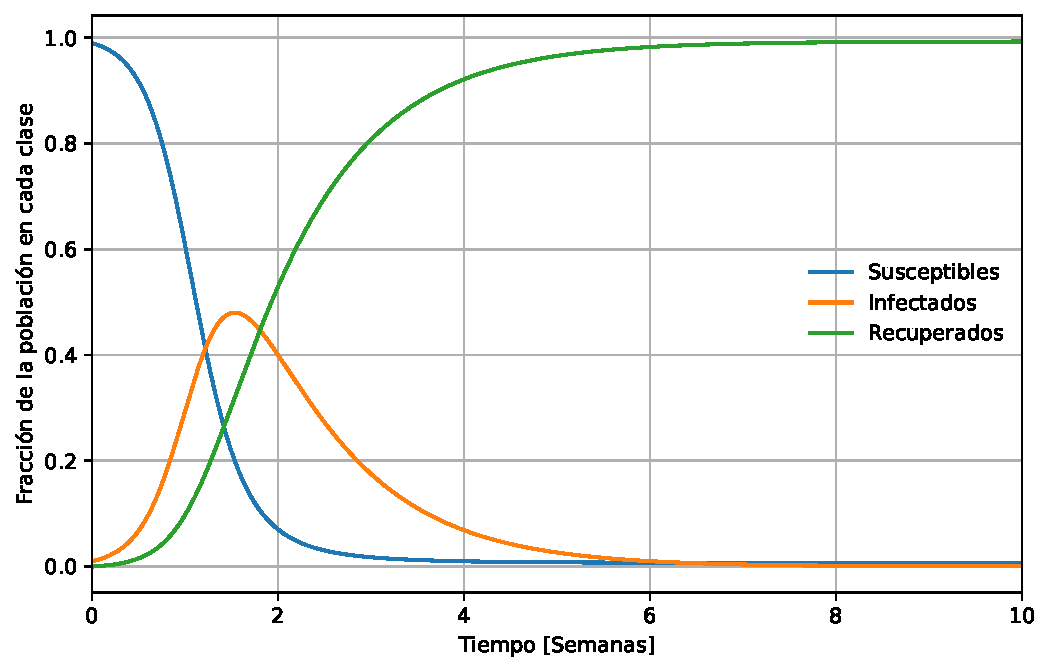
\includegraphics[width=\imsize]{SIR.pdf}
  \caption[Solución numérica del modelo S-I-R]{Evolución temporal de las variables del modelo resuelto numéricamente 
  con $\beta=~5$/semana, $\gamma=1$/semana, $I_0=0.01$ y $S_0=0.99$.}
  \label{fig:SIR}
\end{figure}


Es claro que la figura \ref{fig:SIR} no muestra toda la riqueza del sistema, ya que simplemente muestra la solución para un solo conjunto de parámetros y 
condiciones iniciales. Es decir, es de esperar que la dinámica difiera si por ejemplo la tasa de transmisión $\beta$ es menor. En particular, es de 
interés saber qué conjunto de parámetros $\beta$ y $\gamma$ favorecen o dificultan el progreso de la infección. Esto puede determinarse de manera sencilla pidiendo que $\dv{I}{t}<0$ 
al momento del brote de la infección. De esto resulta que si $S_0<S_c=\gamma/\beta$ para cualquier $I_0>0$ entonces la infección no progresa. 
Este es un resultado conocido, obtenido por Kermack y McKendrick (1927).

El cociente $\gamma/\beta$ es la tasa de recuperación relativa, sin embargo, es más habitual referirse a su recíproco, $R_0=~\beta/\gamma$ 
conocido en epidemiología comúnmente como el número de reproducción básico, el cual describe la media de personas infectadas por un individuo 
infectado durante su estadío infectivo. Dado que usualmente $S_0\approx 1$, la condición para que la infección perezca se lee ahora en función de $R_0$
simplemente como $R_0 < 1$. Lo cual resulta natural: si un infectado infecta en promedio a menos de una persona en lo que cursa la enfermedad entonces 
la infección no se propaga. 

En la figura \ref{fig:SIR_R} se puede ver la evolución temporal de las variables del modelo resuelto numéricamente con distintos 
números de reproducción básico $R_0$. Se observa que en la medida que $R_0 \to 1$ la magnitud del máximo de infección va decreciendo, mientras que cuando $R_0 = 1$ la 
cantidad de infectados solo decrece en el tiempo hasta llegar a cero. Lo mismo sucede si $R_0<1$.

Es importante no confundir el número de reproducción básico $R_0$ con el número de reproducción efectivo $R_e(t)$. El primero considera que todos los individuos de la 
población son susceptibles, mientras que el segundo no y varía con el tiempo, se define como $R_e(t)=\beta S(t)/\gamma$. Este probablemente sea el indicador epidemiológico 
más usado. De manera similar que con $R_0$, se puede ver que si $R_e(t) < 1$ entonces la tasa de infección $\dv{I}{t}\left(t\right)$ es decreciente.

\begin{figure}[t]
  \centering
  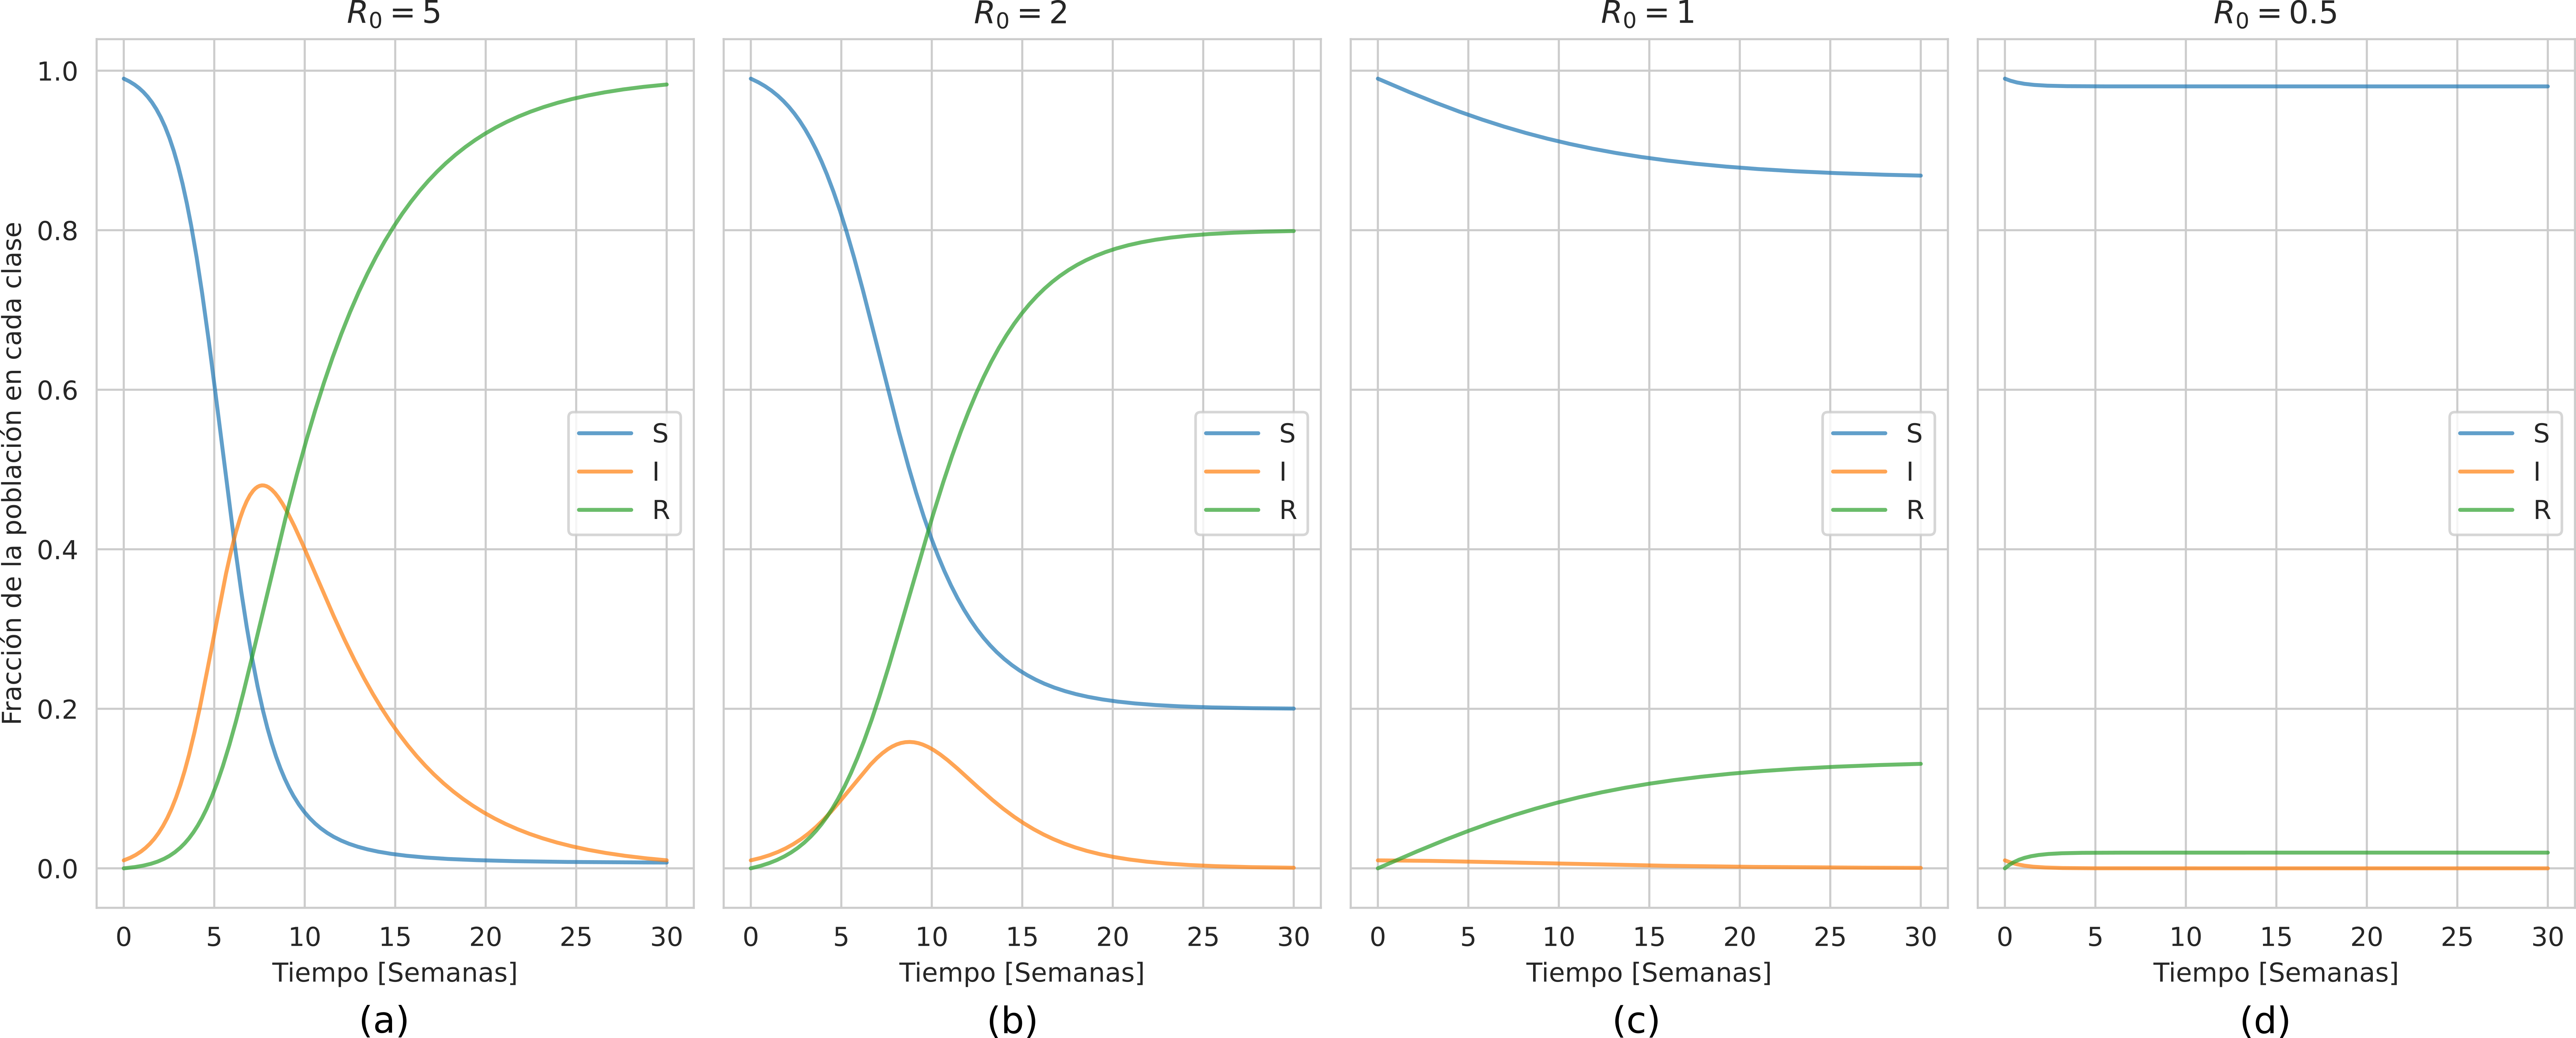
\includegraphics[width=\imsizeL]{SIR_R.png}
  \caption[Solución numérica del modelo S-I-R con distintos valores de $R_0$]{Evolución temporal de las variables del modelo resuelto numéricamente con (a) 
  $R_0 = 5$, (b) $R_0 = 2$, (c) $R_0 = 1$ y (d) $R_0 = 0.5$.}
  \label{fig:SIR_R}
\end{figure}

Otra cantidad de interés es la fracción de la población que no se contagió nunca. Es decir, cuánto vale el límite $\lim_{t \to \infty} S(t) \equiv S(\infty)$. De la figura 
\ref{fig:SIR_R} se puede ver que cuando $R_0=5$ la fracción de la población que no se 
contagia es muy cercana a cero, pero distinta a cero en fin. Mientras que cuando $R_0 = 2$, pareciera que $S(\infty) \to 0.2$. Para responder esta pregunta de manera más 
general podemos tomar la ecuación \ref{Seq}, dividirla por \ref{Req} y luego integrar para obtener una expresión de $S$ en función de $R$. De esto resulta que,
$$S(t) = S_0 e^{-R_0R(t)},$$
tomando el límite correspondiente, usando $\lim_{t \to \infty}R(t)\equiv R(\infty)$ y que $R(\infty) = 1 - S(\infty)$, resulta la siguiente ecuación trascendental 
para $S(\infty)$
\begin{align}
  S(\infty) &= S_0 e^{-R_0 (1 - S(\infty))},\nonumber \\
  0 &= S(\infty) - S_0 e^{-R_0 \left(1 - S(\infty)\right)}.  \label{Sinf}
\end{align}
Puede verse que si $S(\infty) = S_0$, entonces el miembro derecho de \ref{Sinf} es positivo, mientras que si $S(\infty) = 0$, es negativo. De modo que la ecuación 
\ref{Sinf} tiene una solución para $S(\infty)$ entre $0$ y $1$. Es decir, sin importar qué tan grande sea el número de reproducción básico $R_0$, o bien, qué tan 
contagiosa sea la enfermedad, siempre existe una fracción de la población que no se contagia.

Es importante señalar brevemente las virtudes y fundamentalmente las hipótesis bajo las que se presenta este modelo. La ventaja más notable es la 
simplicidad y el carácter didáctico del mismo, que como vimos, permite definir y asimilar conceptos generales asociados a la problemática de manera sencilla.
Esta simplicidad, sin embargo, viene acompañada de hipótesis que en ocasiones resultan restrictivas y poco realistas en lo que respecta a una dinámica
tan compleja como la de una epidemia. Por ejemplo, se ignoran efectos de demografía los cuales
pueden tener un impacto apreciable sobre la dinámica a escalas temporales extensas propias de una endemia. Además, se trata de un modelo de campo medio, 
donde se asume que cada sujeto de la población interactúa con todos los demás, es decir, desprecia heterogeneidades que puedan surgir de la edad, el 
espacio, la movilidad o aspectos de comportamiento. Adicionalmente, supone que individuos que pasaron por la enfermedad adquieren inmunidad para toda la vida y que
un sujeto inmedianamente infectado puede infectar a otro. Por supuesto, esto no desmerece en nada al modelo, el cual sigue siendo extremadamente útil como primera 
aproximación al modelado de este tipo de sistemas complejos, simplemente es importante recordar las hipótesis sobre las que se trabaja para evitar posibles confusiones.

Por último, es de interés mencionar que si bien el enfoque ha estado hasta ahora centrado en una descripción epidemiológica, es posible extender este 
mismo modelo de manera sencilla a otras problemáticas. En particular, puede asociarse rápidamente el modelo SIR con la dinámica
de un incendio en un bosque, donde los <<susceptibles>> son los árboles que pueden incendiarse, los <<infectados>> son los árboles en 
llamas y los <<recuperados>> los árboles que ya han sido quemados y no pueden volver a incendiarse \cite{provatas1995flame,PhysRevE.96.013107,PhysRevLett.79.1515,provatas1995scaling}. O bien, puede asociarse con la dinámica de una 
reacción química, donde los <<susceptibles>> son los reactantes, los <<infectados>> los productos intermedios y los <<recuperados>> los productos finales \cite{ipsen2000amplitude,field1985oscillations,horvath1993instabilities}.
 

\sect{Modelo SIR de reacción-difusión homogéneo}{modeloRDHo}

De manera general las ecuaciones de reacción-difusión sobre un medio isotrópico son aquellas que pueden escriberse como
\begin{equation}
  \pdv{\vb{u}}{t} = \vb{f} + \div(D\grad{\vb{u}}),
\end{equation}
donde $\vb{u}$ es un campo vectorial que dependende de la posición $\mathbf{x}$ y el tiempo $t$, $\vb{f}$ es el término de reacción, que es función de 
$\vb u$, $\vb x$ y $t$, mientras que $\div(D\grad{\vb{u}})$ es el término de difusión, donde D es la matriz de difusión que puede ser función de $\vb x$.
Este tipo de ecuaciones han sido ampliamente estudiadas \cite{keeling:infectious_diseases,Murray2002,Murray2003,crank1979mathematics} y se denominan así porque originalmente 
se utilizaron para estudiar la dinámica de reactivos químicos \cite{turing52the}.

En lo que respecta al modelo SIR de reacción-difusión que nos interesa a nosotros, este puede escribirse de manera sencilla agregando 
el término difusivo a las ecuaciones (\ref{Seq} - \ref{Req}), dejando de lado la ecuación para $R$, esto es 
\begin{align}
  \partial_t S &=-\beta SI + D_{S} \laplacian{S},\label{Seqdif}\\[.3cm]
  \partial_t I &=\beta SI - \gamma I + D_{I} \laplacian{I}.\label{Ieqdif}
\end{align}

Donde ahora $S$, $I$ y $R$ son funciones de la posición $(x,y)$ en un espacio bidimensional además del tiempo $t$, de modo que ahora 
se cumple $S(x,y,t)+I(x,y,t)+R(x,y,t)=1$ para todo $(x,y,t)$. En este nuevo modelo 
(\ref{Seqdif} - \ref{Ieqdif}) los términos difusivos dan lugar a una transmisión local de la infección. Es decir, abandonamos 
el modelo de campo medio que teníamos en la sección \ref{sec:sir_cm} donde todos los individuos podían interactuar entre sí a un instante dado.

Hemos supuesto que los coeficientes de difusión $D_{S}$ y $D_{I}$ son independientes de la posición y que la matriz $D$ es diagonal 
dejando de lado la posibilidad de difusión cruzada. Adicionalmente, tanto $\beta$ como $\gamma$ son 
independientes de la posición, dando lugar a un medio totalmente homogéneo, es decir que todos los puntos del espacio son equivalentes en términos de transmisión. Esta 
es una característica crítica a remarcar, ya que en la sección \ref{sec:modeloRDHe} presentamos el correspondiente modelo heterogéneo, donde 
el medio puede adquirir un carácter desordenado, que es el foco de estudio de este trabajo.

A continuación se muestran algunos resultados interesantes asociados a este modelo que serán de interés a la hora de compararlo con su versión heterogénea.

\ssect{Soluciones de onda}{ondas}

Dada una fracción de infectados inicial $I(x,y,0)$ y una fracción de susceptibles 
distribuída homogéneamete $S(x,y,0)=S_0$, se quiere saber cómo es la evolución espacio-temporal de la fracción de infectados $I(x,y,t)$. En la problemática 
de incendios la idea sería la misma, pero cambiando infectados por, digamos, incendiados. 

Nuevamente, no es posible resolver las ecuaciones \ref{Seqdif} y \ref{Ieqdif} de manera exacta, sin embargo, es posible estudiar qué condiciones deben 
satisfacerse para que cierto tipo de soluciones puedan existir. En particular, nos interesa estudiar bajo qué condiciones podría existir una solución de onda 
y qué características tendría.

Para ello proponemos una solución de onda plana (onda solitaria o frente) donde 
\begin{align}
  S(x,y,t)&=S(z), & I(x,y,t)&=I(z), &  z&=x-ct, \label{wave}
\end{align}
que representa una onda de infección viajando en la dirección $x$ positiva con una velocidad $c>0$. Reemplazando \ref{wave} en \ref{Seqdif} y \ref{Ieqdif}, resulta el 
siguiente sistema de ecuaciones no lineales,

\begin{align}
  D_S S''+ cS'-\beta IS &=0,\label{Sz} \\[.3cm] D_I I'' + cI' + \beta I(S-\gamma/\beta)&=0, \label{Iz}
\end{align}
donde las primas indican derivadas respecto de $z$. Como es habitual, este sistema tampoco puede resolverse explícitamente, sin embargo, imponiendo las 
siguientes condiciones para las soluciones\footnote{Se utiliza la siguiente notación por simplicidad, dada una función $f(z)$, 
\[\lim_{z\to\pm\infty}f(z)\equiv f(\pm\infty)\]}
\begin{align*}
  I(\pm\infty)&=0,   &  S(\infty) &= S_0,  & S(-\infty) &= S_1,   
\end{align*}
donde $S_1$ sería la fracción de susceptibles que deja la onda por detrás, es posible linearizar la ecuación \ref{Iz} para $z$ donde $S(z)\approx S_0$,
es decir, sobre el perfil frontal de la onda. De lo cual resulta,
\begin{equation}
  D_I I'' + cI'+\beta I(S_0-\gamma/\beta)=0,\label{Idez}
\end{equation}
que tiene una solución $I(z)\propto e^{-\lambda z}$, con $\lambda$ satisfaciendo,
\[D_I \lambda^2 - c \lambda +\beta(S_0-\gamma/\beta)=0,\]
es decir,
\[\lambda = \frac{c}{2D_I}\pm \sqrt{(c/2D_I)^2-\frac{\beta}{D_I}(S_0-\gamma/\beta)}.\]
Debemos imponer además que $\lambda \in \mathds R$ con $\lambda>0$, de otra manera la solución no sería autoconsistente. Al imponer que $\lambda>0$ 
resulta $\gamma/\beta<S_0$, que es la misma condición que habíamos obtenido en la sección \ref{sec:sir_cm} para que la infección progrese, 
mientras que ahora es una condición necesaria para la existencia de soluciones onda, las cuales darían lugar a la 
propagación de la infección. Más interesante quizás, es la condición $\lambda \in \mathds{R}$, de la cual resulta que 
\begin{align}
  0\leq&(c/2D_I)^2-\frac{\beta}{D_I}(S_0-\gamma/\beta),\nonumber \\[.3cm]
  c\geq&2\sqrt{D_I(\beta S_0-\gamma)}\equiv c_0, \label{eq:c0}
\end{align}
dando así una velocidad mínima $c_0$ para la existencia de la onda. Veremos en el capítulo \ref{cap:resultados_criticos} que la velocidad de propagación es de hecho
la mínima encontrada aquí $c=c_0$. Tomando esto por cierto, el perfil frontal de la onda de infección queda dado por 
\begin{equation}
  I_f(z)\propto \exp[-\frac{c_0}{2D_I}z].\label{larika2}  
\end{equation}

Haciendo una cuenta equivalente para el perfil posterior de la onda donde $S(z)\approx S_1$, hay que resolver la ecuación análoga a \ref{Idez}, 
$D_I I'' + cI'+\beta I(S_1-\gamma/\beta)=0$, de esto resulta 

\begin{align}
  I_p(z)&\propto \exp[\left(-\frac{c_0}{2D_I}+\sqrt{(c_0/2D_I)^2-\frac{\beta}{D_I}(S_1-\gamma/\beta)}\right)z], \label{larika} \\[.3cm]
  I_p(z)&\propto \exp[\left(-\frac{c_0}{2D_I}+ \sqrt{\frac{\beta}{D_I}(S_0-S_1)}\right)z].
\end{align}
Donde en el último paso se reemplazó la expresión para $c_0$ (ecuación \ref{eq:c0}) dentro de la raiz. De la ecuación \ref{larika} se ve que es necesario que $\gamma/\beta>S_1$, dado que debe satisfacerse $I_p(-\infty) = 0$, de modo que en resumen se tiene la siguiente relación
\[S_0>\gamma/\beta>S_1>0,\]
es decir, que la fracción de susceptibles que quedan tras el paso de la onda no es suficiente para activar una onda de retroceso ya que $S_1<\gamma/\beta$.

En resumen, se obtuvieron expresiones analíticas aproximadas del perfil frontal y posterior que tendría una solución de onda, ecuaciones \ref{larika2} 
y \ref{larika} respectivamente, las cuales dan a entender que el perfil completo de la onda es asimétrico. Se determinó a su vez la velocidad de propagación del frente 
$c_0=2\sqrt{D_I(\beta S_0-\gamma)}$ y se estableció la jerarquía $S_0>\gamma/\beta>S_1>0$ para la existencia del mismo.

Por último, quería comentar brevemente acerca de la estabilidad de estas soluciones. Nótese que en el desarrollo hemos reducido la dimensionaldiad del problema a una dimensión $z$ y hemos mostrado el tipo de soluciones admisibles en esta situación. Sin embargo, estas soluciones solo tienen sentido si pensamos en una condición inicial plana para el campo de infectados. Sin emabrgo, es de interés generalizar un poco más y entender qué sucede si la condición no es plana o si presenta algunas perturbaciones iniciales. En este sentido, decimos que el frente es estable si bajo perturbaciones iniciales el frente tiende a uno plano, mientras que es inestable si no. Puede verse que esta estabilidad está directamente asociada al cociente entre los coeficientes de difusión de infectados y susceptibles $\frac{D_S}{D_I}$. Si $\frac{D_S}{D_I}<1$ entonces el frente es estable, en otro caso es inestable. Nosotros ignoraremos por completo la difusión en susceptibles, es decir, utilizaremos $D_S=0$, por lo cuál siempre estaremos con frentes estables en este sentido. Se decidió así por simplicidad y porque no constituía un objetivo principal investigar los efectos con distintos parámetros de difusión. Sin emabargo, parecía importante mencionarlo dado que no es un efecto trivial y puede incorporar nuevos fenómenos al problema. Para una discusión más detallada acerca de esto puede referirse a Ref. \cite{horvath1993instabilities}.

\ssect{Soluciones en sistema de reacción-difusión-convección}{SIRrdc}

En este trabajo exploramos algunos resultados sobre un modelo SIR como el presentado en la sección \ref{sec:modeloRDHo} pero con un término adicional de convección. Esto es,
\begin{align}
  \partial_t S & = -\beta SI + D_S \laplacian{S} \label{S_eq_v}\\
  \partial_t I &= \beta SI + D_I \laplacian{I}- \mathbf{v} \cdot \nabla I \label{I_eq_v}
\end{align}
donde $\mathbf{v}$ es un campo vectorial. En términos epidemiológicos no es fácil dar una interpretación a este campo vectorial, sin embargo, podría interpretarse 
como un campo de migración de individuos infectados de un lugar a otro y la dirección de $\mathbf{v}$ sería la dirección de la migración, en tanto que su magnitud 
sería la velocidad de migración. Pensando en incendios es más sencillo motivar este término de convección, pues se podría interpretar como el campo de viento. 

Ahora bien, se puede ver que este modelo también tiene soluciones de onda cuando $\mathbf{v}$ es constante. Sin perder generalidad podemos tomar $\mathbf{v}=(v,0)$ con 
$v>0$, de modo que la ecuación de evolución para $I$ queda
\begin{equation}
  \partial_t I = \beta SI + D_I \laplacian{I}- v \partial_x I.
\end{equation}
Pasando las ecuaciones a un sistema de coordenadas que se mueve a velocidad $v$ en $x$-positivo, es decir, $x'=x-vt$, se obtiene 

\begin{equation}
  \partial_t I = \beta SI + D_I \laplacian{I},
\end{equation}
es decir, recuperamos el sistema de reacción-difusión que estudiamos antes. Tomando el desarrollo de la sección anterior se obtiene en este caso que la velocidad de propagación 
del frente de infección es 
$$c = c_0 + v,$$
mientras que si tomamos viento en contra $\mathbf{v} = (-v,0)$ se tiene,
$$c = c_0 - v.$$
Lo interesante del caso con viento en contra es que debemos pedir que $c>0$, dado que buscamos una solución de onda viajando en la dirección $x$-positivo, de lo cual surge un nuevo valor crítico para el umbral de propagación. Es decir,

\begin{align}
  c &> 0 \nonumber \\
  2\sqrt{D_I\beta(S_0-\gamma/\beta)}\ - v &> 0 \nonumber \\
  \sqrt{D_I\beta(S_0-\gamma/\beta)} &> v/2 \nonumber \\
  \beta &> \frac{1}{S_0}(\frac{v^2}{4D_I}+\gamma) \equiv \beta_c 
\end{align}
donde $\beta_c$ corresponde al nuevo umbral de propagación dados $(\gamma,D_I,v,S_0)$ con viento en contra. En contraste, el valor umbral de $\beta$ con viento a favor, que 
corresponde al mismo que en el caso sin viento, es $\beta_c = \frac{\gamma}{S_0}$. En resumen, dado el conjunto de parámetros $(\gamma,D_I,v,S_0)$, la mínima tasa de transmisión
necesaria para la existencia de una solución de onda viajando en la dirección $x$-positivo es

\begin{equation}
  \beta_c = 
  \begin{cases}
    \frac{\gamma}{S_0} \; \text{, si} \; v\geq 0 \\
    \frac{1}{S_0}(\frac{v^2}{4D_I}+\gamma) \; \text{, si} \; v<0.
  \end{cases}
\end{equation}


\sect{Modelo SIR de reacción-difusión-convección heterogéneo}{modeloRDHe}

En esta sección presentamos el modelo completo que estudiamos con profundidad en este trabajo junto a algunas descripciones estadísticas del mismo que se usarán 
posteriormente. 

Esencialmente las ecuaciones son las mismas que \ref{S_eq_v} y \ref{I_eq_v} con la salvedad de que ahora introducimos hetereogeneidad en el medio poniendo 
una tasa de transmisión $\beta_{\vb{r}}$ dependiente de la posición. Por completitud escribimos las ecuaciones nuevamente aquí,
\begin{align}
  \pdv{S}{t}&=-\beta_{\vb{r}} SI + D_{S} \laplacian{S}  ,\label{Seqfinal}\\[.3cm]
  \pdv{I}{t}&=\beta_{\vb{r}} SI - \gamma I + D_{I} \laplacian{I} - \mathbf{v} \cdot \nabla I.\label{Ieqfinal}
\end{align}

Una tasa de transmisión $\beta_{\vb{r}}$ de este tipo podría utilizarse, por ejemplo, para estudiar el efecto de la vacunación sobre la población. Esto es 
entendible dado que se espera que los lugares donde hay población vacunada la tasa de transmisión sea menor ya que hay menos individuos susceptibles para
infectarse. Otra alternativa apuntaría a describir lugares donde la tasa de transmisión es más baja por un efecto de densidad poblacional o lugares donde se toman medidas de prevención. 
En cuanto a la propagación de incendios podría interpretarse de manera similar como una variación de la densidad o el tipo de vegetación en el espacio, lo cual 
facilitaría o no la transmisión de las llamas.

\section{Problema y observables}
\label{Problema}

Vamos a estudiar el frente de infección/incendio en $(x,y,t) \in \Omega \times [0,\infty)$, con $\Omega = [0,L_x] \times [0,L_y]$. Sea la región donde 
comienza la infección/incendio $\Omega_0 = (0,\delta x) \times (0,L_y)$ donde $\delta x \in (0,L_x)$, entonces la condición inicial con la que trabajamos es

\begin{align*}
  I(x,y,0) &= 
  \begin{cases}
  I_0 & \text{si} \; (x,y) \in \Omega_0 \\
  0 & \text{si} \; (x,y) \notin \Omega_0  
  \end{cases}
  & ;&&
  S(x,y,0) &=
  \begin{cases}
  1-I_0 & \text{si} \; (x,y) \in \Omega_0 \\
  S_0 & \text{si} \; (x,y) \notin \Omega_0.
  \end{cases}
\end{align*}
Mientras que las condiciones de contorno son rígidas en la dirección $x$
\begin{align*}
  I(0,y,t)=I(L_x,y,t)=S(0,y,t)=S(L_x,y,t)=0,
\end{align*}
y periódicas en la dirección $y$, 
\begin{align*}
  I(x,0,t)=&I(x,L_y,t) & S(x,0,t)=&S(x,L_y,t). 
\end{align*}
Estas condiciones iniciales y de contorno dan lugar a un único frente de onda propagándose en la dirección $x$, lo cual resulta conveniente para realizar un análisis 
estadístico a partir de ciertos observables, los cuales se definen a continuación.

Para caracterizar las fluctuaciones espaciales y temporales del frente de infección/incendio, definimos primero el campo de desplazamiento del frente $u(y,t)$ como
\begin{equation}
  \max_{x\in(0,L)}\{I(x,y,t)\}=I(u(y,t),y,t).\label{campo}
\end{equation}
Es decir, $u(y,t)$ es la posición en $x$ que maximiza la fracción de infectados/incendiados para un dado $y$ en el instante $t$. Se define a su vez el centro de masa
de $u(y,t)$,
\begin{equation}
  u_{cm}(t)\equiv\langle u(y,t)\rangle_{y},\label{centromasa}
\end{equation}
donde $\langle...\rangle_{y}$ indica el promedio sobre la coordenada $y$. Definimos la amplitud de $I(x,y,t)$ como el valor medio de $I(x,y,t)$ sobre $u(y,t)$, es decir,
\begin{equation}
  I_{max}(t)=\langle I(u(y,t),y,t)\rangle_{y}.\label{maximo}
\end{equation}
Por otro lado, la velocidad del frente se define como
\begin{equation}
  c(t)\equiv\dot{u}_{cm}(t).\label{velocidad}
\end{equation}
Mientras que las fluctuaciones del frente de onda pueden ser caracterizadas definiendo el ancho del mismo $\omega(t)$ como la desviación estándar de $u(y,t)$,
\begin{equation}
  w(t)^2\equiv\langle[u(y,t)-u_{cm}(t)]^2\rangle_{y},\label{rugosidad}
\end{equation}  
o bien utilizando el factor de estructura,
\begin{equation}
  S(q,t)\equiv|u(q,t)|^2,\label{factor}
\end{equation}
donde $u(q,t)$ es la transformada de Fourier sobre el espacio de $u(y,t)$.

En capítulos posteriores utilizaremos los observables definidos aquí como principales herramientas para caracterizar y comparar de manera cuantitativa
los efectos que tienen distintas heterogeneidades, introducidas mediante $\beta_{\vb r}$, sobre la dinámica del problema. A continuación describimos los distintos
tipos de heterogeneidades estudiadas. 

\subsection*{Tipos de heterogeneidades}

Discutiremos aquí brevemente los distintos tipos de heterogeneidad que nos proponemos explorar en este trabajo. Para ello simplemente describimos los distintos 
$\beta_{\vb r}$ utilizados.
\subsubsection*{Heterogeneidad dicotómica-aleatoria (DA)}

Consiste en una tasa de transmisión $\beta_{\vb r}$ espacialmente dicotómica con una distribución de probabilidad dada por 
\begin{equation}
  f(\beta_{\vb r}) = p\delta(\beta_{\vb r}) + (1-p)\delta(\beta_{\vb r}-\beta),\label{prop}
\end{equation}
donde $0\leq p \leq 1$. Esto es equivalente a decir, dada una posición $\vb r = (x,y)$, la tasa de transmisión en $\vb r$ es $0$ con probabilidad $p$ o
es $\beta$ con propabilidad $1-p$. Nótese que cuando $p=0$ se recupera el caso homogéneo,
donde la tasa de transmisión es $\beta$ en todo el espacio. Con la distribución de probabilidad \ref{prop}, 
este $\beta_{\vb r}$ cumple 
\begin{align}
  \overline{\beta_{\vb{r}}}&= (1-p)\beta, \\[.3cm]
  \overline{\beta_{\vb r}\beta_{\vb{r'}}} - \overline{\beta_{\vb{r}}}\;\overline{\beta_{\vb{r'}}} &= \beta^2p(1-p)\delta(\vb r - \vb{r'}),
\end{align}
donde las barras indican valor medio sobre desorden. Puede verse que no se tiene correlación espacial, por tanto se estaría representando una estrategia de vacunación 
aleatoria sobre la población. Llamaremos a la hetereogeneidad definida así como <<heterogeneidad
dicotómica-aleatoria>> o DA simplemente.

Para ganar cierta intuición sobre lo que implica este tipo de heterogeneidad sobre el espacio, en la figura \ref{fig:heterogeneidad_dicotómica_aleatoria} 
pueden verse distintas realizaciones de $\beta_{\vb r}$ para diferentes valores de $p$ representadas sobre una grilla de $20 \times 20$.

\begin{figure}[t]
  \centering
  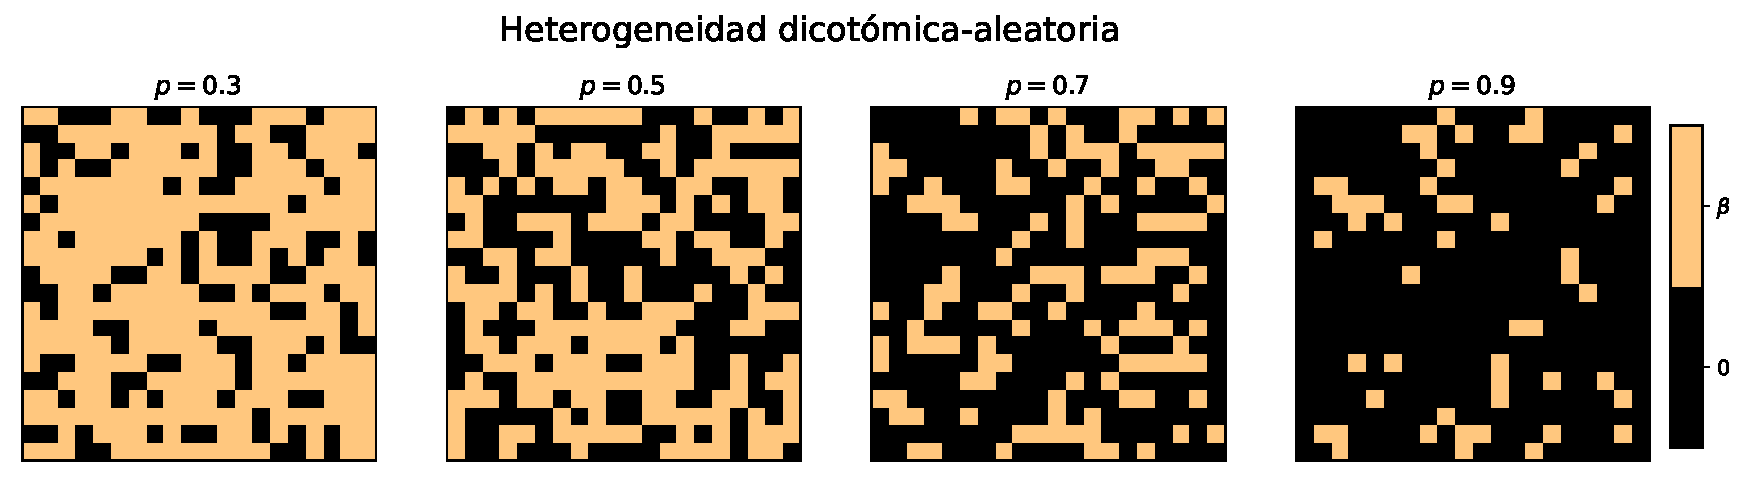
\includegraphics[width=1\textwidth]{heterogeneidad_dicot_aleatoria.pdf}
  \caption{De izquierda a derecha: representación de $\beta_{\vb r}$ sobre una grilla de $20 \times 20$ para  $p=0.3$ , $p=0.5$ , $p=0.7$ y $p=0.9$.}
  \label{fig:heterogeneidad_dicotómica_aleatoria}
\end{figure}

\subsubsection*{Heterogeneidad suavizada (S)}

En este caso se propone una heterogeneidad suavizada, donde, en primera instancia, se genera un $\beta_{\vb r}$ usando la distribución
de probabilidad \ref{prop} y luego se aplica una regla de suavizado $n$ veces. En un esquema discreto donde el espacio de $L\times L$ se descompone en
$N\times N$ cuadrantes de $L/N$ por $L/N$, la regla de suavizado puede describirse de manera recursiva como,
\begin{align}
  \beta^{(0)}_{\vb r} &= \beta_{\vb r}^{DA},\\ 
  \beta^{(n)}_{i,j} &= \frac{1}{5} (\beta^{(n-1)}_{i-1,j} + \beta^{(n-1)}_{i+1,j} + \beta^{(n-1)}_{i,j-1} + \beta^{(n-1)}_{i,j+1} + \beta^{(n-1)}_{i,j}),\label{suavizado}
\end{align}
donde $\beta^{(n)}_{i,j}$ es el valor del nuevo $\beta^{(n)}_{\vb r}$ en el cuadrante $\vb r =(i,j)$ con $i,j = 1,2...,N$.
\footnote{Se consideran condiciones periódicas sobre la grilla, de modo que por ejemplo, $i=N+1$ se entiende como $i=1$.} 

La particularidad de esta
tasa de transmisión es que ahora presenta una correlación espacial local. Esto implica que disminuirán los efectos de cambios abruptos en la tasa de 
transimisión sobre la propagación del frente de onda. Por otro lado, el valor medio de la tasa de transmisión del medio S con $n$ pasos $\overline{\beta^{(n)}_{\vb r}}$ es igual al valor medio de la tasa de transimisión del medio DA que le da origen $\overline{\beta_{\vb r}^{DA}}$. Esto puede verse por inducción, $\overline{\beta^{(1)}_{\vb r}}=\overline{\beta^{(0)}_{\vb r}}=\overline{\beta_{\vb r}^{DA}}$,
luego, asumiendo que $\overline{\beta^{(n-1)}_{\vb r}}=\overline{\beta_{\vb r}^{DA}}$ resulta que $\overline{\beta^{(n)}_{\vb r}}=\overline{\beta_{\vb r}^{DA}}$.

\begin{figure}[t]
  \centering
  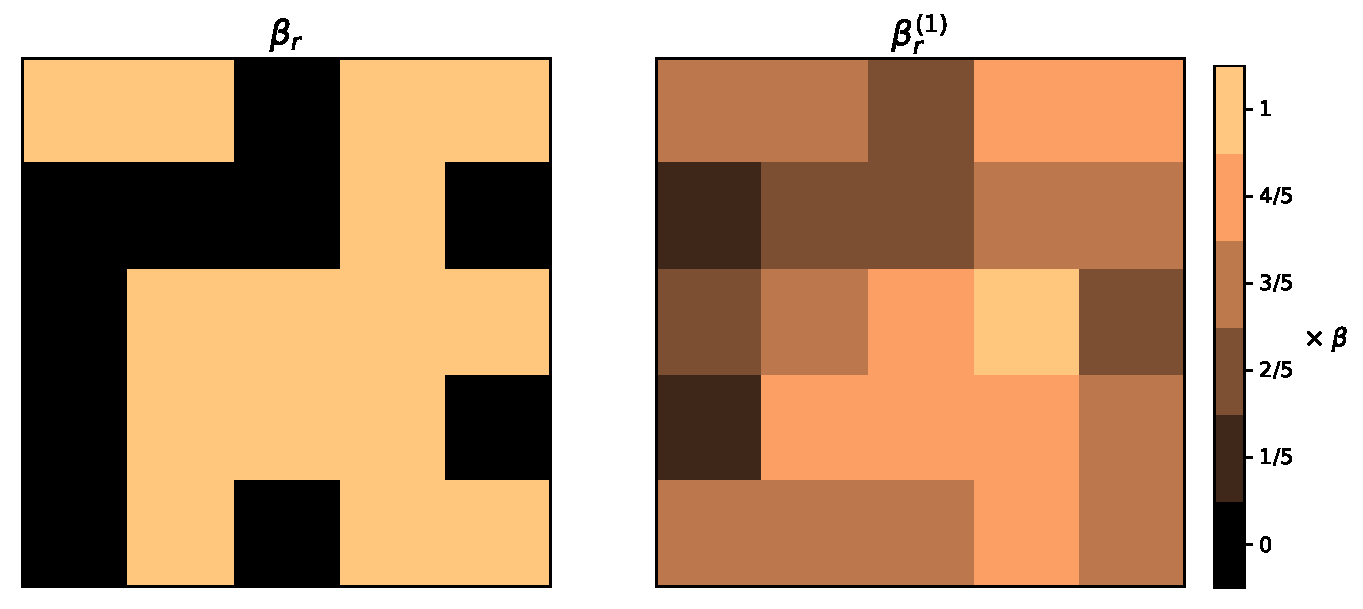
\includegraphics[width=.6\textwidth]{smoth_step.pdf}
  \caption{A la izquierda, se muestra una realización de $\beta_{\vb r}^{DA}$ con $p=0.5$. A la derecha, se muestra el efecto de un paso de suavizado 
  sobre el $\beta_{\vb r}^{DA}$ original generando $\beta_{\vb r}^{(1)}$.}
  \label{fig:smoth_step}
\end{figure}

En la figura \ref{fig:smoth_step} puede verse esquemáticamente el efecto de un paso de suavizado sobre una grilla de $10\times10$, mientras que 
en la figura \ref{fig:smoth} se muestran realizaciones de $\beta^{(1)}_{\vb r}$ para diferentes $p$ sobre una grilla de $20\times20$, compare con 
la figura \ref{fig:heterogeneidad_dicotómica_aleatoria}.

\begin{figure}[!b]
  \centering
  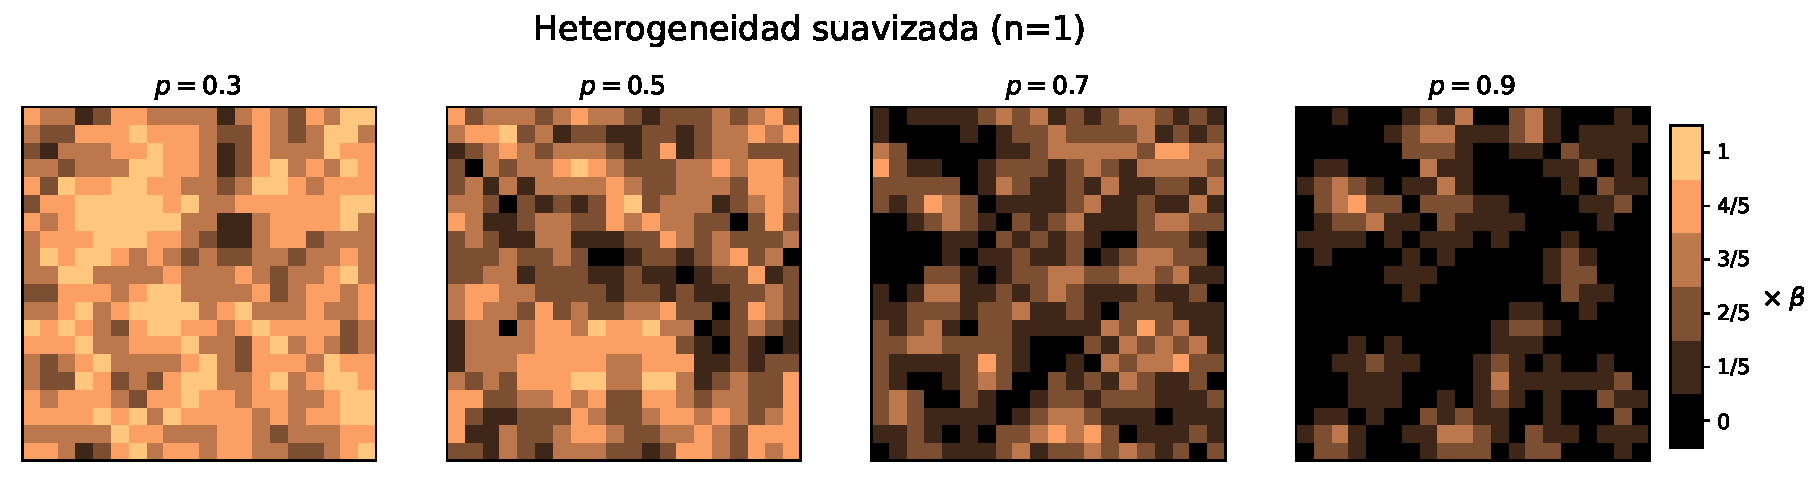
\includegraphics[width=.9\textwidth]{het_suav.pdf}
  \caption{Representación de $\beta^{(1)}_{\vb r}$ sobre una grilla de $20 \times 20$ para  $p=0.3$ , $p=0.5$ , $p=0.7$ y $p=0.9$.}
  \label{fig:smoth}
\end{figure}
\begin{figure}[!b]
  \centering
  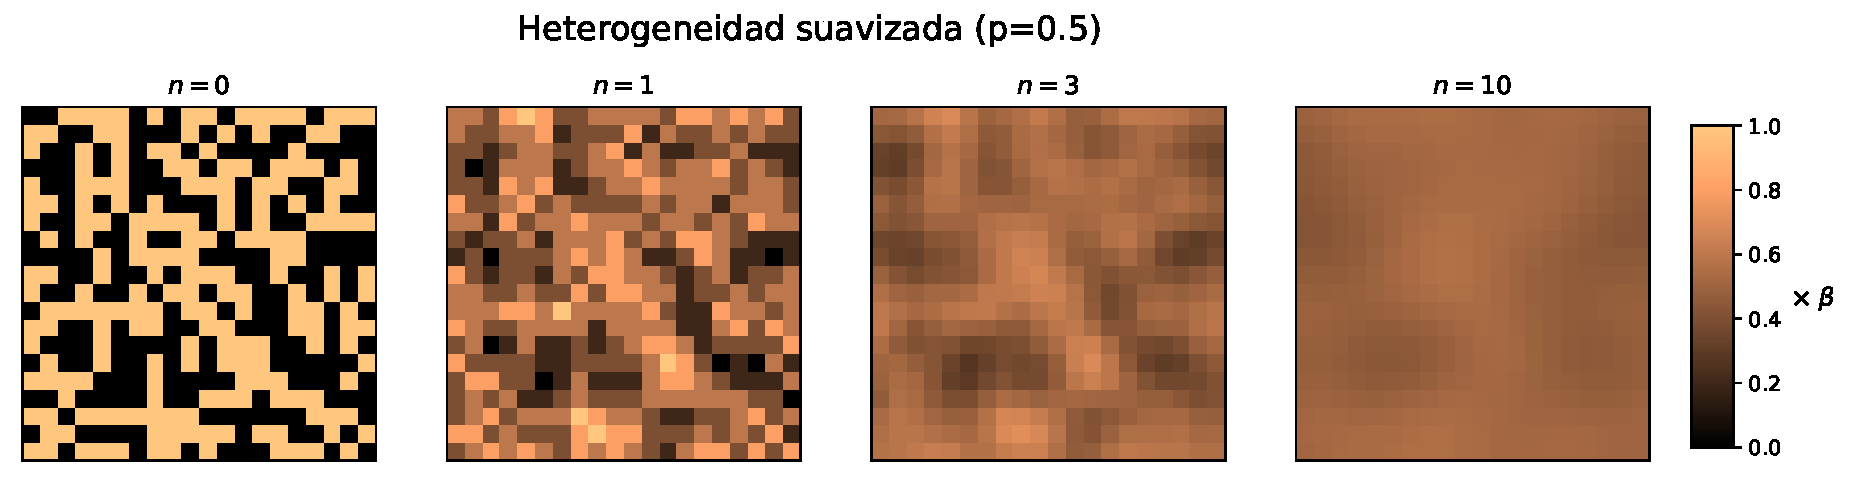
\includegraphics[width=.9\textwidth]{nsmoth_step.pdf}
  \caption{Se muestran los $\beta^{(n)}_{\vb r}$ con $n=0,1,3,10$ sobre una grilla de $20\times20$.}
  \label{fig:nsmoth_step}
\end{figure}

Un detalle más a notar sobre este tipo de heterogeneidad es que para $n\rightarrow\infty$ recuperamos el caso
homogéneo, con una tasa de transmisión constante de valor $\overline{\beta_{\vb r}}=~(1-p)\beta$. Esto puede verse tomando el límite en la ecuación \ref{suavizado} para $n\rightarrow\infty$, poniendo 
$\lim_{n\to \infty}\beta^{(n)}_{i,j}\equiv\beta^{(\infty)}_{i,j}$, se tiene
\[
  4\beta^{(\infty)}_{i,j} = \beta^{(\infty)}_{i-1,j} + \beta^{(\infty)}_{i+1,j} + \beta^{(\infty)}_{i,j-1} + \beta^{(\infty)}_{i,j+1},
\]
para todo $(i,j)$, de modo que la única posibilidad es que $\beta^{(\infty)}_{i,j}$ sea el mismo para todo $(i,j)$ e igual a $\overline{\beta_{\vb r}}$, ya que debe
conservar el valor medio. En la figura \ref{fig:nsmoth_step} se muestra el efecto al realizar varios pasos de suavizado.


\vspace*{-.5cm}
\subsubsection*{Heterogeneidad dicotómica-correlacionada (DC)}

Esta consiste, de alguna manera, en una combinación de las dos anteriores. Se genera un $\beta^{(n)}_{\vb r}$ de la misma manera que para la versión 
suavizada. Una vez obtenido este $\beta^{(n)}_{\vb r}$ definimos un nuevo $\tilde{\beta}^{(n)}_{\vb r}$ de la siguiete manera,
\begin{align*}
  \tilde{\beta}^{(n)}_{i,j} &= \beta, \; \;\;\; \mbox{si}\; \beta^{(n)}_{i,j}\geq\overline{\beta_{\vb r}}=(1-p)\beta,  \\
  \tilde{\beta}^{(n)}_{i,j} &= 0,  \;\;\;\;\mbox{si}\; \beta^{(n)}_{i,j}<\overline{\beta_{\vb r}}=(1-p)\beta.
\end{align*}

Este caso presenta correlación local en una versión dicotómica, pero naturalmente no conserva el valor medio. En la figura \ref{fig:smoth_dic} se muestran 
realizaciones para distintos valores de $p$ con $n=1$. Puede observarse a simple viste que la densidad de puntos negros no aumenta con $p$ como 
pasaba en los casos anteriores, esto quiere decir que $p$ no puede interpretarse como la fracción de lugares donde $\beta$ se anula para este caso. Esta diferencia sustancial debe tenerse en cuenta a la hora de comparar resultados entre heterogeneidades. Para ello utilizaremos el valor medio espacial de la tasa de transimsión
$\langle\beta_{\vb r}\rangle_{\vb r} = \beta_m$ en lugar de $p$, ya que da cuenta de esta variación del comportamiento.

En la figura \ref{fig:smoth_dic_step} se muestra el efecto de los pasos de suavizado para este caso con $p=0.5$. En este caso, al hacer el límite 
$n\to \infty$ se recupera nuevamente el caso homogéneo pero con un valor medio de $\tilde{\beta}^{(\infty)}_{\vb r}$ igual a $\beta$.
\begin{figure}[h]
  \centering
  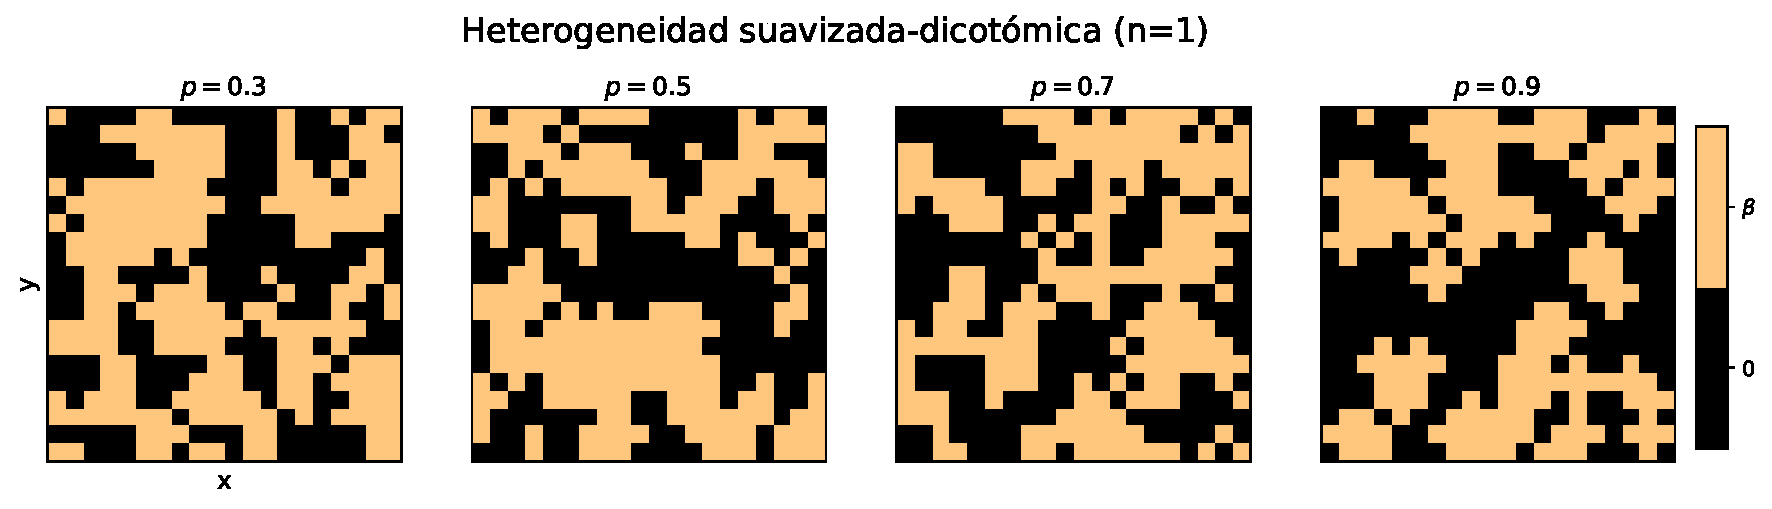
\includegraphics[width=.9\textwidth]{het_suav_dico.pdf}
  \caption{Representación de $\tilde{\beta}^{(1)}_{\vb r}$ sobre una grilla de $20 \times 20$ para  $p=0.3$ , $p=0.5$ , $p=0.7$ y $p=0.9$.}
  \label{fig:smoth_dic}  
\end{figure}
\begin{figure}[h]
  \centering
  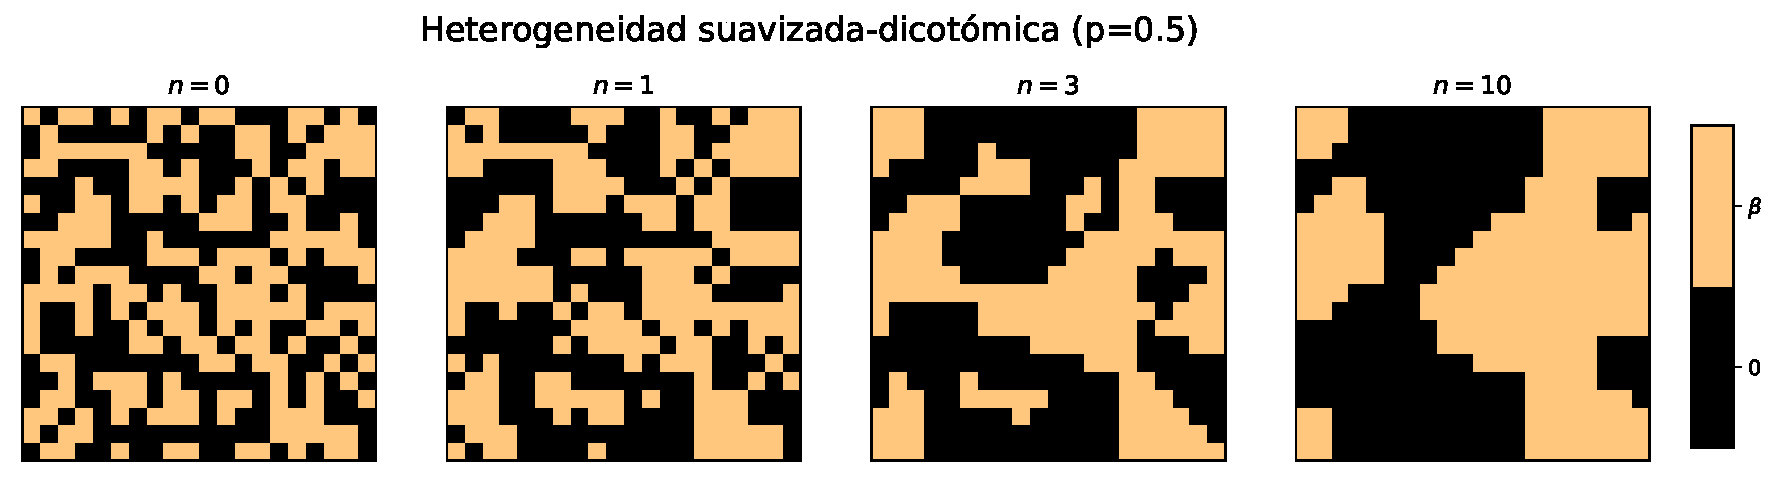
\includegraphics[width=.9\textwidth]{nsmoth_dic_step.pdf}
  \caption{Se muestran los $\tilde{\beta}^{(n)}_{\vb r}$ con $n=0,1,3,10$ sobre una grilla de $20\times20$.}
  \label{fig:smoth_dic_step}
\end{figure}








%\chapter{Conclusiones}
\graphicspath{{figs/}}
\label{Conclusiones}
\vspace*{-.1cm}

Se utilizaron herramientas estadísticas y computacionales para caracterizar frentes de onda gobernados por ecuaciones de reacción-difusión asociadas al modelo SIR sobre 
una variedad de medios estadísticamente isotrópicos. Estos frentes de onda son característicos de diversas fenomenologías asociadas a ecuaciones de reacción-difusión.

En particular, en el ámbito epidemiológico, modelar el efecto que tiene el carácter heterogéneo de la distribución espacial de las poblaciones sobre la dinámica 
infecciosa constituye un desafío complejo y sin lugar a dudas moderno.\cite{RILEY201568}

El trabajo desarrollado aquí constituye un paso en esa dirección. Fue posible 
obtener resultados no triviales respecto de la influencia del medio sobre los frentes de propagación. Características de interés como la velocidad de propagación, la 
amplitud media, la rugosidad del campo de desplazamiento e incluso la nocividad de los frentes fueron desarrolladas a nivel cuantitativo. Exponentes críticos asociados 
a un cambio radical de la dinámica fueron determinados sobre los distintos medios.

Por otro lado, en el modelado de incendios forestales es claro que la topografía, el carácter heterogéneo del medio y las condiciones climáticas son factores 
determinantes. Estos podrían introducirse en el modelo a partir de una interpretación precisa de los efectos que las variaciones en el medio tienen sobre la dinámica y 
ser estudiados utilizando las mismas herramientas desarrolladas aquí.

Es importante notar que exponentes críticos tal como los determinados en este trabajo, suelen estar asociados a una dada clase de universalidad, que resulta independiente 
de los detalles propios del problema estudiado aquí. \cite{barabasi1995fractal} Esto daría la posibilidad de estudiar sistemas más complejos dentro de la misma clase de universalidad a partir 
del modelo más simple que se ha explorado en este trabajo.

Para futuros trabajos en esta línea sería interesante investigar los efectos de la dinámica sobre medios hiper-uniformes, tanto ordenados como desordenados. Así como 
medios con configuraciones periódicas o bien tan arbitrarias como se quiera. También se propone trabajar con medios dinámicos y no solo estacionarios como los estudiados
aquí.


\appendix
\chapter{Metodología numérica}
\label{C:ap1}
\graphicspath{{figs/}}


El sistema de ecuaciones dado por
\begin{align*}
    \pdv{S}{t}&=-\beta_{\vb{r}} SI + D_{S} \laplacian{S},\\[.3cm]
    \pdv{I}{t}&=\beta_{\vb{r}} SI - \gamma I + D_{I} \laplacian{I},
\end{align*}
se resolvió numéricamente utilizando el siguiente esquema explícito de Euler:

\begin{align*}
    S^{n+1}_{ij} &= S^n_{ij} + \Delta t\left( -\beta_{ij} S^n_{ij}I^n_{ij} + \frac{D_{S}}{d^2} (S^n_{i+1j}+S^n_{i-1j}+S^n_{ij+1}+S^n_{ij-1}-4S^n_{ij})\right)\\[.3cm]
    I^{n+1}_{ij} &= I^n_{ij} + \Delta t\left( \beta_{ij} S^n_{ij}I^n_{ij} - \gamma I^n_{ij} + \frac{D_{I}}{d^2} (I^n_{i+1j}+I^n_{i-1j}+I^n_{ij+1}+I^n_{ij-1}-4I^n_{ij})\right) 
\end{align*}
donde los índices $i$ y $j$ corresponden a la discretización de las coordenadas espaciales y el índice $n$ corresponde a la discretización temporal.
Se utilizaron de manera general los siguientes parámetros $\Delta t=0.1$, $d=1$, $D_{I}=1$ y $D_{S}=0$. Los demás parámetros involucrados se indican 
según corresponde en el texto.

Este esquema se implementó por computación en paralelo utilizando procesadores gráficos. De esta manera fue posible resolver de manera eficiente cientos de sistemas 
sobre grillas de $1024\times1024$. En particular se utilizó la librería de \texttt{Python} para computación en paralelo llamada \texttt{\href{https://cupy.dev/}{CuPy}},
que es un equivalente de la librería \texttt{\href{https://numpy.org/}{NumPy}} pero integrada con \texttt{\href{https://developer.nvidia.com/cuda-toolkit}{CUDA}}.

A continuación se muestra la función central del esquema numérico que permite recorrer la grilla del sistema en paralelo y calcular las derivadas del sistema en 
cada nodo utilizando esta librería, se representan a $S$ e $I$ como $X$ e $Y$ respectivamente:\newpage

\begin{lstlisting}[basicstyle=\tiny]
    forces = cp.ElementwiseKernel(
    'raw float64 X, raw float64 Y, raw float64 params,raw float64 beta,raw float64 gamma, int16 L' ,
    'float64 fX,float64 fY',
    '''
    double N = params[0]; double nu = params[1]; double mu = params[2]; double Dx = params[3];
    double Dy = params[4];
    
    int x = i % L;
    int y = (int) i/L;

    fX =  nu - beta[i]*X[i]*Y[i]/N - mu*X[i] + 
        Dx*(X[(x+1)%L + L*y] + X[(x-1+L)%L+L*y] + X[x + L*((y+1)%L)] + X[x + L*((y-1+L)%L)] - 4*X[i]);

    fY = beta[i]*X[i]*Y[i]/N - (gamma[i]+mu)*Y[i] + 
        Dy*(Y[(x+1)%L + L*y] + Y[(x-1+L)%L+L*y] + Y[x + L*((y+1)%L)] + Y[x + L*((y-1+L)%L)] - 4*Y[i]);
    ''',
    'forces')
\end{lstlisting}

y el paso de Euler se lee simplemente como:

\begin{lstlisting}[basicstyle=\tiny]
    ...
    forces(X,Y,params,beta,gamma,Lx,fX,fY)
    X = X + tstep*fX
    Y = Y + tstep*fY
    ...
\end{lstlisting}

Para dar una idea de la aceleración dada por la programación en paralelo, en la figura \ref{gpuvscpu} se muestra el tiempo necesario para resolver un sistema 
de $N\times N$ sitios y $1000$ pasos de Euler con procesadores gráficos (GPU) y con procesadores convencionales (CPU). La diferencia es notable, por ejemplo, 
para un sistema de $1024\times1024$,
el tiempo necesario para resolverlo con CPU es aproximadamente de 2.7 horas, mientras que con GPU se resuelve en 1 segundo. Se muestra también un ajuste 
para ambas curvas del tipo $t\propto N^a$ con $a\approx2$ para ambos. De todo esto resulta clara la necesidad de trabajar con computación en paralelo 
para obtener los resultados desarrollados en este trabajo en un tiempo razonable. Para ver más detalles acerca del código y 
las herramientas computacionales implementadas puede acceder al siguiente 
\textit{\href{https://colab.research.google.com/drive/1r0242WjJD_a5SR3ppiUQG25x4ODiM4Ps?usp=sharing}{Notebook}} de \textit{Google Colab}.

\begin{figure}[h]
    \centering
    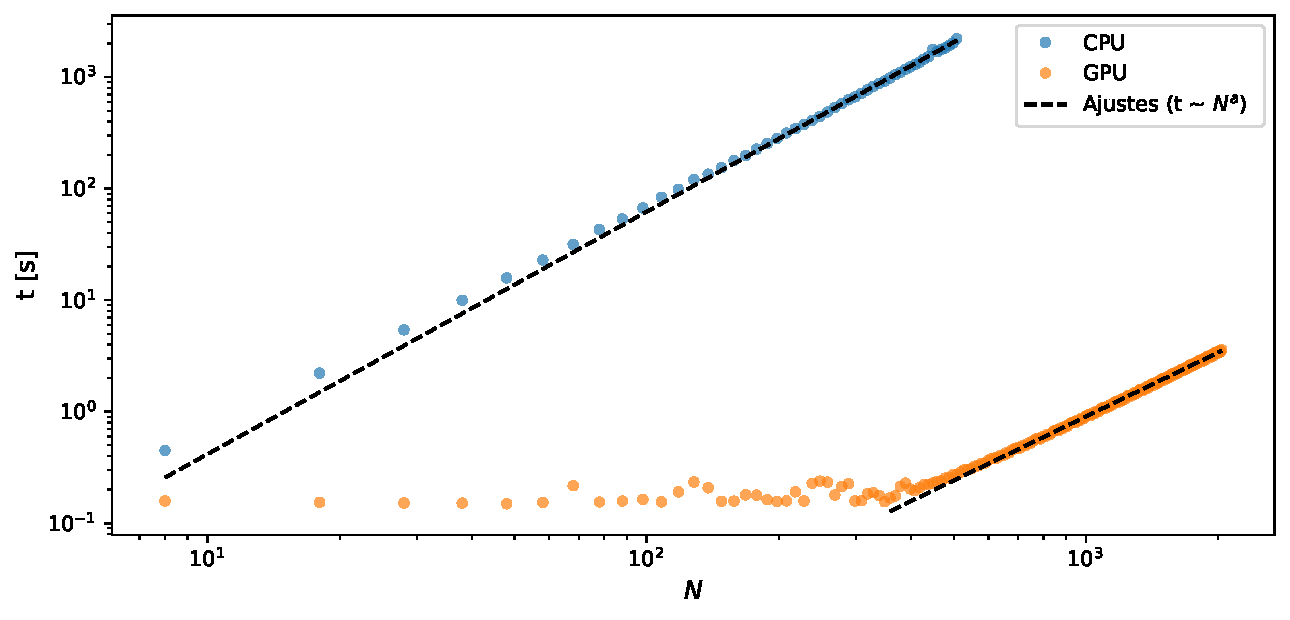
\includegraphics[width=0.8\textwidth]{t_vs_N.pdf}
    \caption{Tiempo de resolución de un sistema de $N\times N$ sitios y 1000 pasos de Euler con procesadores gráficos (GPU) y con procesadores convencionales (CPU). Se muestran 
    también los ajustes de tipo $t\propto N^a$ con $a\approx2$ para ambos.}
    \label{gpuvscpu}
\end{figure}



\begin{biblio}
\bibliography{mibib}
\end{biblio}

\begin{postliminary}

\begin{seccion}{Agradecimientos}
Agradezco al Instituto Balseiro, a la Universidad Nacional de Cuyo y a la Comisión Nacional de Energía Atómica por hacer posible mis estudios universitarios. 
Agradezco enteramente a todo el personal de estas instituciones que hacen posible, con gran esfuerzo y a pesar todas las complicaciones dadas por la pandemia, que 
educación universitaria de altísimo nivel, pública y gratuita llegue a todo el país. Particular agradecimiento para mi director de tesis, Dr. Alejandro Kolton, 
por su gran apoyo en el desarrollo de este trabajo y buena predisposición para todo. Agradezco también a mis compañeros de camada Amir Zablotsky, Pedro \textit{El Bata}
Llauradó, Esteban \textit{El Leches} Acerbo, Marco Madile, Ezequiel Saidman, Martín Famá y Francisco \textit{El Bbto} Gymnich por estar siempre presentes y ayudar a 
liberar las tensiones de la vida universitaria.
\end{seccion}

\end{postliminary}

\end{document}

